% ==============================================================================
% main.tex
% Documento raiz — Relatório Técnico-Científico
% Classe: abntex2 | Compilador: pdflatex + bibtex (Overleaf / TeX Live)
% ==============================================================================

\documentclass[
  12pt,
  oneside,
  a4paper,
  english,
  brazil
]{abntex2}

% --- Pacotes, estilos TikZ, listings e ambiente Quadro ---
% ==============================================================================
% config/pacotes.tex
% Pacotes, estilos tipográficos, TikZ, listagens de código e float Quadro
% Compatível com pdflatex + abntex2 (Overleaf e TeX Live padrão)
% ==============================================================================

% --- Codificação e fontes ---
\usepackage[T1]{fontenc}
\usepackage[utf8]{inputenc}
\usepackage{lmodern}
\usepackage{indentfirst}
\usepackage{microtype}
\usepackage{xcolor}
\usepackage{graphicx}

% --- Matemática e símbolos ---
\usepackage{amsmath}
\usepackage{amssymb}

% --- Tabelas ABNT / IBGE e Quadros ---
\usepackage{booktabs}
\usepackage{array}
\usepackage{tabularx}
\usepackage{multirow}
\usepackage{ragged2e}

% Coluna tabularx com alinhamento à esquerda sem hifenização excessiva
\newcolumntype{L}{>{\RaggedRight\arraybackslash}X}
\newcolumntype{C}{>{\Centering\arraybackslash}X}

% --- Citações e referências (abntex2cite) ---
\usepackage[alf, abnt-etal-list=3]{abntex2cite}

% --- Paleta sóbria de engenharia (para diagramas TikZ e listagens) ---
\definecolor{wegblue}{RGB}{0, 87, 157}
\definecolor{slateink}{RGB}{38, 50, 56}
\definecolor{steelbg}{RGB}{244, 247, 250}
\definecolor{tealnode}{RGB}{0, 121, 107}
\definecolor{amberwarn}{RGB}{217, 119, 6}
\definecolor{crimsonalert}{RGB}{185, 28, 28}
\definecolor{codebg}{RGB}{248, 249, 251}
\definecolor{codeborder}{RGB}{203, 213, 225}
\definecolor{codecomment}{RGB}{100, 116, 139}
\definecolor{codestring}{RGB}{15, 118, 110}

% --- Diagramas vetoriais nativos em TikZ (apenas bibliotecas padrão) ---
\usepackage{tikz}
\usetikzlibrary{
  arrows.meta,
  positioning,
  shapes.geometric,
  fit,
  backgrounds,
  calc,
  decorations.pathreplacing
}

% --- Listagens de código com suporte UTF-8 completo em pdflatex ---
\usepackage{listings}

\lstset{
  basicstyle=\linespread{0.92}\selectfont\ttfamily\scriptsize\color{black},
  backgroundcolor=\color{codebg},
  frame=single,
  rulecolor=\color{codeborder},
  numbers=left,
  numberstyle=\tiny\color{black},
  numbersep=7pt,
  tabsize=2,
  breaklines=true,
  breakatwhitespace=true,
  showstringspaces=false,
  captionpos=t,
  xleftmargin=12pt,
  xrightmargin=4pt,
  aboveskip=3pt,
  belowskip=3pt,
  columns=flexible,
  keepspaces=true,
  commentstyle=\normalfont\color{black},
  keywordstyle=\normalfont\color{black},
  stringstyle=\color{black},
  literate=
    {á}{{\'a}}1 {à}{{\`a}}1 {â}{{\^a}}1 {ã}{{\~a}}1
    {é}{{\'e}}1 {ê}{{\^e}}1 {í}{{\'i}}1
    {ó}{{\'o}}1 {ô}{{\^o}}1 {õ}{{\~o}}1 {ú}{{\'u}}1
    {ç}{{\c{c}}}1
    {Á}{{\'A}}1 {À}{{\`A}}1 {Â}{{\^A}}1 {Ã}{{\~A}}1
    {É}{{\'E}}1 {Ê}{{\^E}}1 {Í}{{\'I}}1
    {Ó}{{\'O}}1 {Ô}{{\^O}}1 {Õ}{{\~O}}1 {Ú}{{\'U}}1
    {Ç}{{\c{C}}}1
    {º}{{\textordmasculine}}1 {ª}{{\textordfeminine}}1
    {°}{{\textdegree}}1 {–}{{--}}1 {—}{{---}}1
}

% Linguagem IEC 61131-3 Structured Text (ST)
\lstdefinelanguage{IECST}{
  morekeywords={
    PROGRAM, END_PROGRAM, VAR, VAR_INPUT, VAR_OUTPUT, END_VAR,
    IF, THEN, ELSIF, ELSE, END_IF, CASE, OF, END_CASE,
    FOR, TO, DO, END_FOR, WHILE, END_WHILE,
    AND, OR, NOT, XOR, MOD, TRUE, FALSE,
    BOOL, INT, UINT, DINT, WORD, DWORD, REAL, TIME, TON, R_TRIG,
    SEL, SHL, BOOL_TO_WORD, UINT_TO_TIME
  },
  sensitive=false,
  morecomment=[l]{//},
  morecomment=[s]{(*}{*)},
  morestring=[b]'
}

% Linguagem JavaScript (nó function do Node-RED)
\lstdefinelanguage{JavaScript}{
  morekeywords={
    const, let, var, function, return, if, else, for, of, in,
    new, try, catch, throw, true, false, null, undefined, Math, Date, Object, Array,
    msg, flow, global, node, context
  },
  sensitive=true,
  morecomment=[l]{//},
  morecomment=[s]{/*}{*/},
  morestring=[b]",
  morestring=[b]'
}

% Linguagem JSON / JSON Schema
\lstdefinelanguage{JSON}{
  morekeywords={true, false, null},
  sensitive=true,
  morestring=[b]"
}

% Linguagem SQL (PostgreSQL DDL)
\lstdefinelanguage{PGSQL}{
  morekeywords={
    CREATE, TABLE, INDEX, ON, IF, NOT, EXISTS, PRIMARY, KEY, REFERENCES,
    BIGSERIAL, BIGINT, INTEGER, SMALLINT, BOOLEAN, DOUBLE, PRECISION,
    TEXT, VARCHAR, TIMESTAMPTZ, JSONB, DEFAULT, NOW, CHECK, IN, NULL, DESC
  },
  sensitive=false,
  morecomment=[l]{--},
  morecomment=[s]{/*}{*/},
  morestring=[b]'
}

% --- Ambiente float 'quadro' nativo do memoir/abntex2 ---
\newcommand{\quadroname}{Quadro}
\newcommand{\listofquadrosname}{Lista de quadros}
\newfloat[chapter]{quadro}{loq}{\quadroname}
\newlistof{listofquadros}{loq}{\listofquadrosname}
\newlistentry{quadro}{loq}{0}
\setfloatadjustment{quadro}{\centering}
\counterwithout{quadro}{chapter}
\renewcommand{\cftquadroname}{\quadroname\space}
\renewcommand*{\cftquadroaftersnum}{\hfill--\hfill}
\setfloatlocations{quadro}{htbp}

% Numeração contínua para figuras e tabelas
\counterwithout{figure}{chapter}
\counterwithout{table}{chapter}

% --- Padronização tipográfica do texto acadêmico ---
% O texto corrido permanece sem negrito; títulos estruturais são formatados
% pela classe abntex2 e mantêm a hierarquia visual prevista pelo modelo.
\renewcommand{\textbf}[1]{#1}

% --- Espaçamento e parágrafos conforme ABNT ---
\setlength{\parindent}{1.25cm}
\setlength{\parskip}{0pt}
\setlength{\emergencystretch}{3em}

% --- Configuração de cores para links do PDF (sóbrio para impressão/leitura) ---
\pdfstringdefDisableCommands{%
  \def\uppercase#1{#1}%
  \def\MakeUppercase#1{#1}%
  \def\MakeTextUppercase#1{#1}%
}
\makeatletter
\hypersetup{
  colorlinks=true,
  linkcolor=black,
  citecolor=black,
  filecolor=black,
  urlcolor=black,
  bookmarksdepth=4
}
\AtBeginDocument{%
  \hypersetup{
    pdftitle={\imprimirtitulo},
    pdfauthor={\autorespdf},
    pdfsubject={Documento Técnico -- Pipeline de Análise de Dados com WEG PLC500, Modbus TCP/IP e Node-RED},
    pdfkeywords={WEG PLC500, CODESYS, Modbus TCP/IP, Node-RED, Pipeline de Dados, FastAPI, Machine Learning, LLM, Indústria 4.0}
  }%
}
\makeatother


% --- Metadados institucionais centralizados ---
% ==============================================================================
% config/metadados.tex
% Metadados institucionais centralizados
% ==============================================================================

\titulo{Arquitetura e Especificação Técnica de uma Pipeline Híbrida de Análise de Dados Industriais Integrando WEG PLC500, Comunicação Modbus TCP/IP e Orquestração com Node-RED}

\autor{Augusto P. Dantas \and Gabriel Simão \and Gabriel Silvano}
\newcommand{\autorespdf}{Augusto P. Dantas, Gabriel Simão, Gabriel Silvano}

\local{Jaraguá do Sul -- SC}

\data{2026}

\instituicao{Centroweg Senai}

\tipotrabalho{Relatório Técnico}

\orientador[Coordenador:]{Lucas de Sousa Santos}

% --- Identificação técnica do documento ---
\newcommand{\codigorelatorio}{RT-AUT-2026-001}
\newcommand{\versaorelatorio}{Revisão 1.0}
\newcommand{\classificacaodoc}{Documentação de Engenharia e Arquitetura}

\preambulo{%
  Relatório técnico desenvolvido no escopo de Situação de Aprendizagem de
  Internet das Coisas (IoT) no Centroweg Senai, apresentando a arquitetura, a
  especificação, a implementação completa e a validação por simulação em gêmeo
  digital de uma pipeline híbrida de análise de dados industriais integrando
  controlador lógico programável WEG PLC500 programado em \textit{Structured Text}
  (IEC~61131-3) via CODESYS, comunicação Modbus TCP/IP, orquestração em cinco
  abas no Node-RED, inferência de aprendizado de máquina via FastAPI e
  \textit{scikit-learn}, diagnóstico por modelo de linguagem restrito por
  JSON Schema Draft 2020-12 e persistência relacional em PostgreSQL.%
}


% --- Customização da capa e folha de rosto ---
% ==============================================================================
% pretextual/folha_rosto_capa.tex
% Customização da Capa e Folha de Rosto conforme ABNT NBR 10719:2015
% ==============================================================================

% --- Capa conforme ABNT NBR 10719:2015 ---
\renewcommand{\imprimircapa}{%
  \begin{capa}%
    \center
    {\ABNTEXchapterfont\large\imprimirinstituicao}

    \vspace*{1.5cm}

    {\ABNTEXchapterfont\large\imprimirautor}

    \vfill

    \begin{center}
      \ABNTEXchapterfont\bfseries\LARGE\imprimirtitulo
    \end{center}

    \vspace*{0.8cm}

    {\normalsize\codigorelatorio\ -- \versaorelatorio}

    \vfill

    {\large\imprimirlocal}
    \par
    {\large\imprimirdata}
    \vspace*{1cm}
  \end{capa}%
}

% --- Folha de rosto conforme ABNT NBR 10719:2015 ---
\makeatletter
\renewcommand{\folhaderostocontent}{%
  \begin{center}
    {\ABNTEXchapterfont\large\imprimirinstituicao}

    \vspace*{1.2cm}

    {\ABNTEXchapterfont\large\imprimirautor}

    \vspace*{\fill}\vspace*{\fill}

    \begin{center}
      \ABNTEXchapterfont\bfseries\Large\imprimirtitulo
    \end{center}

    \vspace*{0.6cm}

    {\small\textbf{Identificação:} \codigorelatorio\ (\versaorelatorio) \quad|\quad \textbf{Classificação:} \classificacaodoc}

    \vspace*{\fill}

    \abntex@ifnotempty{\imprimirpreambulo}{%
      \hspace{.45\textwidth}
      \begin{minipage}{.5\textwidth}
        \SingleSpacing
        \imprimirpreambulo
      \end{minipage}%
      \vspace*{\fill}
    }%

    {\abntex@ifnotempty{\imprimirorientador}{%
      \imprimirorientadorRotulo~\imprimirorientador\par
    }}

    \vspace*{\fill}

    {\large\imprimirlocal}
    \par
    {\large\imprimirdata}
    \vspace*{1cm}
  \end{center}
}
\makeatother


% ==============================================================================
\begin{document}

% Seleciona idioma português do Brasil como principal
\selectlanguage{brazil}

% Retira espaço extra obsoleto entre frases e aplica espaçamento acadêmico
\frenchspacing
\OnehalfSpacing
\setlength{\parskip}{0pt}
\setlength{\parindent}{1.25cm}

% ------------------------------------------------------------------------------
% ELEMENTOS PRÉ-TEXTUAIS
% ------------------------------------------------------------------------------
\pretextual

% Capa
\imprimircapa

% Folha de rosto (sem ficha catalográfica no verso em modo oneside)
\imprimirfolhaderosto*

% Resumo em língua vernácula
% ==============================================================================
% pretextual/resumo.tex
% Resumo em língua vernácula
% ==============================================================================

\setlength{\absparsep}{18pt}
\begin{resumo}
Este documento técnico apresenta a arquitetura, a especificação de engenharia, a implementação completa e a validação automatizada de uma pipeline híbrida de aquisição, análise de dados e atuação para automação industrial e Internet das Coisas (IoT), desenvolvida no âmbito de uma Situação de Aprendizagem (SA) no Centroweg Senai. Concebido inicialmente como um servidor de tempo \textit{Network Time Protocol} (NTP) baseado em microcontrolador ESP32 e receptor \textit{Global Navigation Satellite System} (GNSS), o projeto teve seu escopo integralmente redefinido após limitações práticas de recepção satelital em ambiente interno de laboratório (\textit{indoor}) e restrições de infraestrutura inviabilizarem o protótipo original, validando-se junto à coordenação a transição para uma bancada de Internet Industrial das Coisas (IIoT) autocontida e reproduzível. Na camada de campo (24\,Vcc PNP), documentada com esquemáticos elétricos em KiCad~8 e CircuiTikZ, quatro botoeiras (\texttt{B1} a \texttt{B4}) simulam sensores de presença de peça, nível crítico, sobretemperatura e parada de emergência normalmente fechada (\textit{fail-safe}), enquanto quatro LEDs (\texttt{L1} a \texttt{L4}) com resistores limitadores de 2,2\,k$\Omega$ representam motor, válvula de alívio, alarme e indicação de operação normal. Na camada de controle, programada de forma modular em \textit{Structured Text} (IEC~61131-3) no CODESYS~V3.5 (\texttt{GVL\_Modbus}, \texttt{FB\_\allowbreak Debounce\allowbreak Counter}, \texttt{FB\_\allowbreak Watchdog\allowbreak Heartbeat}, \texttt{FB\_\allowbreak Safety\allowbreak Interlock} e \texttt{PLC\_PRG} com ciclo de varredura de 10\,ms e exportação PLCopen TC6 XML v2.01), o CLP WEG PLC500 opera como servidor Modbus TCP/IP na porta 502 com filtro de \textit{debounce} de 50\,ms, contadores de eventos, \textit{watchdog} por \textit{heartbeat} e intertravamento determinístico local. Na camada de orquestração e análise, uma aplicação Node-RED~v4 estruturada em cinco abas utiliza o pacote \texttt{node-red-\allowbreak contrib-\allowbreak modbus} para realizar \textit{polling} a 500\,ms (2\,Hz) de 23 registradores de base zero, persistir séries temporais e auditorias no PostgreSQL~16 (quatro tabelas e três visões operacionais) e computar atributos estatísticos em janelas deslizantes de 60\,s com passo (\textit{stride}) de 15\,s. Esses vetores alimentam um microsserviço de aprendizado de máquina em FastAPI e \textit{scikit-learn} --- composto por detector de anomalias \texttt{Isolation\allowbreak Forest} e classificador supervisionado \texttt{HistGradient\allowbreak Boosting\allowbreak Classifier} treinados sobre 18\,h de telemetria a 2\,Hz (129.600 amostras brutas e 3.688 janelas com lacunas de purga $\ge 60$\,s) --- acoplado a um agente baseado em Modelo de Linguagem Grande (LLM) restrito por \textit{JSON Schema} Draft 2020-12 e guardião de monotonicidade de segurança. Por fim, a solução é verificada integralmente em malha fechada (\textit{Software-in-the-Loop}) nos dez casos de teste (\texttt{CT-01} a \texttt{CT-10}) por meio de um gêmeo digital Modbus TCP de 10\,ms (\texttt{plc\_\allowbreak simulator.py}).

\textbf{Palavras-chave}: Internet Industrial das Coisas. WEG PLC500. Modbus TCP/IP. Node-RED. Aprendizado de máquina. Gêmeo digital.
\end{resumo}


% Abstract em língua estrangeira
% ==============================================================================
% pretextual/abstract.tex
% Resumo em língua estrangeira (Abstract)
% ==============================================================================

\begin{resumo}[Abstract]
\begin{otherlanguage*}{english}
This technical report presents the architecture, engineering specification, complete implementation, and automated validation of a hybrid data acquisition, analytics, and actuation pipeline for industrial automation and the Internet of Things (IoT), developed within an IoT Learning Situation (\textit{Situação de Aprendizagem}) at Centroweg Senai. Originally conceived as a Network Time Protocol (NTP) server based on an ESP32 microcontroller and a Global Navigation Satellite System (GNSS) receiver, the project underwent a complete scope pivot after indoor satellite reception constraints and laboratory infrastructure limitations rendered the initial prototype unfeasible, leading to a formally approved transition toward a self-contained and reproducible Industrial IoT (IIoT) testbed. At the 24\,VDC PNP field layer, documented through KiCad~8 and CircuiTikZ schematics, four pushbuttons (\texttt{B1} to \texttt{B4}) simulate part presence, critical level, overtemperature, and normally closed fail-safe emergency stop sensors, while four Light-Emitting Diodes (\texttt{L1} to \texttt{L4}) with 2.2\,k$\Omega$ current-limiting resistors represent the motor drive, relief valve, alarm indicator, and normal operation status. At the control layer, modularly programmed in Structured Text (IEC~61131-3) within CODESYS~V3.5 (\texttt{GVL\_Modbus}, \texttt{FB\_\allowbreak Debounce\allowbreak Counter}, \texttt{FB\_\allowbreak Watchdog\allowbreak Heartbeat}, \texttt{FB\_\allowbreak Safety\allowbreak Interlock}, and \texttt{PLC\_PRG} running at a 10\,ms scan cycle and exported as PLCopen TC6 XML v2.01), the WEG PLC500 Programmable Logic Controller operates as a Modbus TCP/IP server on port 502 with 50\,ms input debouncing, event counters, a heartbeat communication watchdog, and local deterministic safety interlocking. At the orchestration and analytics layer, a five-tab Node-RED~v4 application uses the \texttt{node-red-\allowbreak contrib-\allowbreak modbus} package to poll 23 zero-based registers every 500\,ms (2\,Hz), persist telemetry and audit trails in PostgreSQL~16 (four tables and three operational views), and compute statistical features over 60\,s sliding windows with a 15\,s stride. These feature vectors feed a FastAPI and \textit{scikit-learn} machine learning microservice---comprising an \texttt{Isolation\allowbreak Forest} anomaly detector and a supervised \texttt{HistGradient\allowbreak Boosting\allowbreak Classifier} trained on 18\,h of 2\,Hz telemetry (129,600 raw samples and 3,688 windows separated by $\ge 60$\,s purge gaps)---coupled with a Large Language Model (LLM) diagnostic agent constrained by JSON Schema Draft 2020-12 validation and a monotonicity safety guard. Finally, the complete architecture is verified through automated Software-in-the-Loop testing across ten test cases (\texttt{CT-01} to \texttt{CT-10}) driven by a 10\,ms Modbus TCP digital twin (\texttt{plc\_\allowbreak simulator.py}).

\vspace{\onelineskip}
\noindent
\textbf{Keywords}: Industrial Internet of Things. WEG PLC500. Modbus TCP/IP. Node-RED. Machine learning. Digital twin.
\end{otherlanguage*}
\end{resumo}


% Lista de ilustrações
\pdfbookmark[0]{\listfigurename}{lof}
\listoffigures*
\cleardoublepage

% Lista de tabelas
\pdfbookmark[0]{\listtablename}{lot}
\listoftables*
\cleardoublepage

% Lista de quadros (códigos, matrizes e casos de teste)
\pdfbookmark[0]{\listofquadrosname}{loq}
\listofquadros*
\cleardoublepage

% Lista de abreviaturas e siglas
% ==============================================================================
% pretextual/siglas.tex
% Lista de abreviaturas e siglas (ordem alfabética)
% ==============================================================================

\begin{siglas}
  \item[ADU] \textit{Application Data Unit} (Unidade de Dados de Aplicação)
  \item[API] \textit{Application Programming Interface} (Interface de Programação de Aplicações)
  \item[CLP] Controlador Lógico Programável
  \item[CPU] \textit{Central Processing Unit} (Unidade Central de Processamento)
  \item[DDL] \textit{Data Definition Language} (Linguagem de Definição de Dados)
  \item[DI] \textit{Digital Input} (Entrada Digital)
  \item[DO] \textit{Digital Output} (Saída Digital)
  \item[ETH] \textit{Ethernet} (Interface de Rede Ethernet)
  \item[FC] \textit{Function Code} (Código de Função Modbus)
  \item[GNSS] \textit{Global Navigation Satellite System} (Sistema Global de Navegação por Satélite)
  \item[IEC] \textit{International Electrotechnical Commission} (Comissão Eletrotécnica Internacional)
  \item[IHM] Interface Homem-Máquina
  \item[IIoT] \textit{Industrial Internet of Things} (Internet Industrial das Coisas)
  \item[IoT] \textit{Internet of Things} (Internet das Coisas)
  \item[IP] \textit{Internet Protocol} (Protocolo de Internet)
  \item[IT] \textit{Information Technology} (Tecnologia da Informação)
  \item[JSON] \textit{JavaScript Object Notation}
  \item[LED] \textit{Light-Emitting Diode} (Diodo Emissor de Luz)
  \item[LLM] \textit{Large Language Model} (Modelo de Linguagem Grande)
  \item[MBAP] \textit{Modbus Application Protocol} (Cabeçalho do Protocolo de Aplicação Modbus)
  \item[ML] \textit{Machine Learning} (Aprendizado de Máquina)
  \item[NA] Normalmente Aberto
  \item[NF] Normalmente Fechado
  \item[NMEA] \textit{National Marine Electronics Association} (Padrão de Sentenças de Navegação)
  \item[NTP] \textit{Network Time Protocol} (Protocolo de Tempo de Rede)
  \item[OT] \textit{Operational Technology} (Tecnologia de Operação)
  \item[PDU] \textit{Protocol Data Unit} (Unidade de Dados de Protocolo)
  \item[PLC] \textit{Programmable Logic Controller} (Controlador Lógico Programável)
  \item[PNP] \textit{Positive-Negative-Positive} (Lógica de Acionamento Tipo Fonte / \textit{Sourcing})
  \item[PPS] \textit{Pulse Per Second} (Pulso por Segundo)
  \item[RTT] \textit{Round-Trip Time} (Tempo de Ida e Volta)
  \item[SA] Situação de Aprendizagem
  \item[SCADA] \textit{Supervisory Control and Data Acquisition}
  \item[SQL] \textit{Structured Query Language} (Linguagem de Consulta Estruturada)
  \item[ST] \textit{Structured Text} (Texto Estruturado -- IEC 61131-3)
  \item[TCP] \textit{Transmission Control Protocol} (Protocolo de Controle de Transmissão)
  \item[TLS] \textit{Transport Layer Security}
  \item[VLAN] \textit{Virtual Local Area Network} (Rede Local Virtual)
  \item[WD] \textit{Watchdog} (Temporizador de Supervisão de Comunicação)
\end{siglas}


% Lista de símbolos
% ==============================================================================
% pretextual/simbolos.tex
% Lista de símbolos utilizados nas formulações técnicas e estatísticas
% ==============================================================================

\begin{simbolos}
  \item[$T_p$] Período de varredura (\textit{polling}) do cliente Modbus TCP/IP no Node-RED ($\text{ms}$)
  \item[$T_{db}$] Tempo de filtragem de \textit{debounce} digital das botoeiras no PLC500 ($\text{ms}$)
  \item[$T_{wd}$] Limiar de tempo máximo (\textit{timeout}) do \textit{watchdog} de \textit{heartbeat} ($\text{ms}$)
  \item[$W$] Duração da janela temporal deslizante para agregação analítica ($\text{s}$)
  \item[$N_i(W)$] Número de bordas de subida (acionamentos) do sensor $i$ na janela $W$
  \item[$\lambda_i(W)$] Taxa de acionamento do sensor $i$ na janela $W$ ($\text{eventos/min}$)
  \item[$D_i(W)$] Proporção de tempo em estado ativo (\textit{duty cycle}) do sensor $i$ na janela $W$
  \item[$\mu_i$] Média histórica da taxa de acionamento do sensor $i$ em regime nominal
  \item[$\sigma_i$] Desvio-padrão histórico da taxa de acionamento do sensor $i$
  \item[$z_i(W)$] Escore padronizado (\textit{Z-score}) de anomalia para o sensor $i$ na janela $W$
  \item[$\epsilon$] Constante positiva de regularização numérica para evitar divisão por zero
\end{simbolos}


% Sumário
\pdfbookmark[0]{\contentsname}{toc}
\tableofcontents*
\cleardoublepage

% ------------------------------------------------------------------------------
% ELEMENTOS TEXTUAIS
% ------------------------------------------------------------------------------
\textual

% ==============================================================================
% capitulos/01_introducao.tex
% Capítulo 1 — Introdução
% ==============================================================================

\chapter{Introdução}
\label{cap:introducao}

\section{Contextualização}
\label{sec:contextualizacao}

A transformação digital dos ambientes fabris, impulsionada pelo paradigma da Indústria 4.0, pela Internet das Coisas (IoT) e pela sua vertente industrial (IIoT), tem aproximado de forma crescente os sistemas de Tecnologia de Operação (OT) das plataformas de Tecnologia da Informação (IT). Historicamente, Controladores Lógicos Programáveis (CLPs) operavam confinados em redes de campo isoladas, dedicados exclusivamente ao controle sequencial, ao intertravamento de máquinas e à supervisão local \cite{moraes_castrucci}. Nas arquiteturas conectadas modernas, entretanto, espera-se que esses controladores atuem como nós inteligentes de borda (\textit{edge devices}), expondo variáveis operacionais em tempo quase real para pipelines analíticas capazes de identificar anomalias, sintetizar diagnósticos contextualizados e retroalimentar ações supervisórias ao processo \cite{chandola_2009, stouffer_nist_ot}.

Controladores de nova geração como o WEG PLC500 --- programável em ambiente CODESYS conforme a norma IEC 61131-3 e equipado com duas interfaces Gigabit Ethernet independentes com suporte nativo ao protocolo Modbus TCP/IP --- oferecem uma ponte robusta entre o chão de fábrica e serviços de software modernos \cite{weg_plc500_manual, iec_61131_3}. Paralelamente, ferramentas de programação visual orientadas a fluxos de eventos (\textit{flow-based programming}), com destaque para o Node-RED, consolidaram-se em soluções de IoT e automação pela facilidade de integração com protocolos industriais por meio do pacote \texttt{node-red-contrib-modbus}, conectividade com bancos de dados relacionais e capacidade de orquestrar serviços analíticos e modelos de Inteligência Artificial (IA) \cite{nodered_docs, nodered_contrib_modbus}.

\section{Histórico do Projeto, Redefinição de Escopo e Enquadramento na Situação de Aprendizagem}
\label{sec:historico_ntp}

Este projeto desenvolve-se no âmbito de uma Situação de Aprendizagem (SA) de Internet das Coisas (IoT) de escopo livre, cuja diretriz pedagógica permite a proposição de arquiteturas e problemas reais de engenharia desde que submetidos à aprovação prévia do professor responsável. Esse formato metodológico visa estimular a autonomia projetual, a capacidade de diagnóstico de viabilidade técnica e a integração ponta a ponta entre hardware, protocolo de comunicação em rede, processamento de dados e atuação.

Dentro dessa modalidade de escopo livre, a proposta inicial submetida ao docente tinha um tema distinto no domínio de redes e sistemas embarcados conectados: o desenvolvimento de um servidor de tempo \textit{Network Time Protocol} (NTP) Stratum~1 utilizando uma antena de recepção \textit{Global Navigation Satellite System} (GNSS) acoplada a um microcontrolador ESP32 \cite{rfc5905_ntp, espressif_esp32}. Na concepção original, o receptor GNSS forneceria ao ESP32 tanto as sentenças de navegação no padrão NMEA (via interface serial UART) quanto o pulso elétrico de sincronismo de alta precisão \textit{Pulse Per Second} (PPS) por interrupção de hardware, permitindo ao microcontrolador disciplinar seu relógio local e atender requisições NTPv4 na rede local.

Durante a fase inicial de avaliação experimental e prototipação em laboratório, contudo, identificaram-se restrições práticas severas que inviabilizaram a continuidade e a validação confiável do servidor NTP em ambiente acadêmico:
\begin{enumerate}
  \item Inviabilidade de recepção de sinal GNSS em ambiente interno (\textit{indoor}): os sinais de radiofrequência transmitidos pelas constelações GNSS na banda~L chegam à superfície terrestre com potência extremamente baixa (tipicamente inferior a $-125\,\text{dBm}$). No interior do laboratório, a atenuação provocada pelas lajes de concreto armado e pela estrutura metálica da edificação impedia a aquisição de efemérides e o travamento (\textit{3D fix}) de satélites suficientes para habilitar o sinal PPS, enquanto medições próximas a janelas sofriam forte degradação por multicaminho (\textit{multipath}).
  \item Limitações de infraestrutura física e de hardware: a instalação permanente de uma antena GNSS ativa externa no telhado do prédio, interligada ao laboratório por cabo coaxial de baixa perda com proteção contra surtos, mostrou-se impraticável dentro das restrições físicas e logísticas do ambiente, somando-se a dificuldades de disponibilidade e estabilidade dos módulos periféricos do protótipo com ESP32.
\end{enumerate}

Diante desse diagnóstico técnico, realizou-se uma pivotagem completa de tema, redirecionando o projeto para um sistema de Internet Industrial das Coisas (IIoT) e análise de dados integralmente reproduzível e validável em bancada \textit{indoor}, sem dependência de visada externa para satélites. Em estrita observância às regras da Situação de Aprendizagem de IoT de escopo livre, o novo escopo --- fundamentado no controlador industrial WEG PLC500 integrado via Modbus TCP/IP à plataforma Node-RED, com botoeiras simulando sensores de campo e indicadores LED simulando atuadores --- foi formalmente apresentado e contou com a aprovação prévia do professor, o que garante plena conformidade do projeto com o estabelecido para a avaliação da disciplina. Ademais, um princípio técnico relevante da proposta original foi preservado na nova arquitetura: o rigor com a consistência temporal das amostras (\textit{timestamping}) e com a avaliação analítica de eventos em janelas de tempo bem definidas.

\section{Definição do Problema e Motivação}
\label{sec:problema}

Na arquitetura adotada após a redefinição de escopo, a integração entre uma pipeline analítica com recursos de IA no Node-RED e um CLP industrial impõe dois desafios centrais de engenharia:

\begin{enumerate}
  \item Fidelidade de simulação segura em bancada: antes do acoplamento a motores de potência, válvulas pressurizadas ou processos térmicos reais, é indispensável dispor de uma bancada didático-industrial controlada que represente os sinais discretos de campo por meio de botoeiras e LEDs em 24\,Vcc, permitindo exercitar trepidação mecânica de contatos, condição de nível crítico, sobretemperatura, parada de emergência e desconexão de rede sem risco físico.
  \item Convivência entre análise inteligente não determinística e segurança determinística: fluxos executados na camada IT --- incluindo \textit{polling} sobre TCP/IP, consultas a banco de dados e chamadas a Modelos de Linguagem Grandes (LLMs) --- apresentam latência variável e comportamento probabilístico. Por conseguinte, toda decisão analítica deve ser validada por contratos de dados estritos (\textit{JSON Schema}) e permanecer subordinada a uma camada determinística de intertravamento \textit{fail-safe} executada localmente no WEG PLC500 \cite{stouffer_nist_ot}.
\end{enumerate}

A motivação deste trabalho reside em documentar uma solução de engenharia completa que enderece ambos os problemas, combinando a confiabilidade determinística do WEG PLC500, a padronização do protocolo Modbus TCP/IP e a capacidade de orquestração e análise híbrida do Node-RED.

\section{Objetivos}
\label{sec:objetivos}

\subsection{Objetivo Geral}
Especificar e implementar a arquitetura técnica, os contratos de comunicação, a lógica determinística de controle, a pipeline analítica híbrida (estatística, aprendizado de máquina via FastAPI/scikit-learn e diagnóstico cognitivo via LLM) e a verificação automatizada \textit{Software-in-the-Loop} (SIL) de um sistema de supervisão de sensores simulados por botoeiras em um controlador WEG PLC500 integrado via Modbus TCP/IP à plataforma Node-RED.

\subsection{Objetivos Específicos}
\begin{itemize}
  \item Definir e documentar um cenário didático-industrial estruturado sobre as entradas e saídas digitais nativas de 24\,Vcc PNP do WEG PLC500 (quatro botoeiras simulando sensores de processo e quatro LEDs com resistores de $2{,}2\,\text{k}\Omega$ simulando atuadores e sinalizadores), contemplando lógica normalmente fechada (NF) para parada de emergência e artefatos completos de engenharia de hardware (\texttt{hardware/bom.csv}, \texttt{hardware/wiring\_table.md}, diagramas CircuiTikZ/TikZ e esquemático KiCad~8 \texttt{plc500\_bench.kicad\_sch}).
  \item Especificar a topologia de rede OT/IT segmentada e o mapa completo de 23 registradores Modbus TCP/IP em endereçamento base zero (\textit{Discrete Inputs}, \textit{Coils}, \textit{Input Registers} e \textit{Holding Registers}), incluindo mecanismo de \textit{heartbeat} e \textit{watchdog} de comunicação.
  \item Implementar a lógica determinística modular no WEG PLC500 em \textit{Structured Text} (IEC 61131-3) no CODESYS V3.5 (\texttt{GVL\_Modbus.st}, \texttt{FB\_DebounceCounter.st}, \texttt{FB\_WatchdogHeartbeat.st}, \texttt{FB\_SafetyInterlock.st} e \texttt{PLC\_PRG.st}, exportados também em formato PLCopen TC6 XML v2.01), abrangendo filtragem de \textit{debounce}, contadores modulares de 16~bits, máquina de estados finitos e intertravamento local com precedência absoluta sobre comandos remotos.
  \item Desenvolver a pipeline analítica híbrida em cinco abas na plataforma Node-RED v4 com o pacote \texttt{node-red-contrib-modbus}, combinando persistência em PostgreSQL~16, extração de atributos em janelas deslizantes de $60\,\text{s}$ (\textit{stride} de $15\,\text{s}$), microsserviço de inferência em aprendizado de máquina via FastAPI e scikit-learn (\texttt{IsolationForest} e \texttt{HistGradientBoostingClassifier}), diagnóstico contextual via agente LLM governado por \textit{JSON Schema} Draft 2020-12 e emissão automática de relatórios operacionais.
  \item Estabelecer e verificar o plano formal de validação (\texttt{CT-01} a \texttt{CT-10}) utilizando um gêmeo digital Modbus TCP determinístico com ciclo de varredura de $10\,\text{ms}$ (\texttt{plc\_simulator.py}), critérios quantitativos de aceitação e matriz de análise de riscos técnicos.
\end{itemize}

\section{Escopo, Delimitações e Conformidade com a Situação de Aprendizagem}
\label{sec:escopo}

Por tratar-se de uma Situação de Aprendizagem de IoT de escopo livre com aprovação prévia do professor, a conformidade do projeto com o estabelecido é assegurada simultaneamente no plano formal (validação docente prévia da redefinição de escopo após os ensaios preliminares de bancada) e no plano técnico-pedagógico, uma vez que a solução contempla de ponta a ponta todas as camadas estruturantes de um ecossistema IoT/IIoT:
\begin{itemize}
  \item Sensoriamento, atuação física e controle de borda (\textit{Edge/OT}): aquisição digital em 24\,Vcc PNP com filtragem de \textit{debounce} ($50\,\text{ms}$), contagem modular de eventos, máquina de estados e intertravamento local \textit{fail-safe} no WEG PLC500, acompanhada de documentação elétrica executiva em KiCad~8 e CircuiTikZ;
  \item Conectividade e interoperabilidade em rede: comunicação cliente/servidor sobre Ethernet segmentada (\texttt{ETH2}) utilizando protocolo aberto Modbus TCP/IP na porta~502 com supervisão contínua de enlace (\textit{heartbeat}/\textit{watchdog});
  \item Orquestração, persistência e processamento analítico híbrido (\textit{IT/IoT Platform}): fluxos orientados a eventos em cinco abas no Node-RED (\texttt{node-red-\allowbreak contrib-\allowbreak modbus}), armazenamento histórico e forense em PostgreSQL~16 (quatro tabelas e três visões operacionais), detecção estatística e inferência supervisionada/não supervisionada via FastAPI (\texttt{Isolation\allowbreak Forest} com ROC-AUC de teste de $0{,}8993$ e \texttt{HistGradient\allowbreak Boosting\allowbreak Classifier} com acurácia de $99{,}73\%$ e Macro-F1 de $0{,}9956$ sobre conjunto sintético de $18\,\text{h}$ a $2\,\text{Hz}$ totalizando $129.600$ amostras brutas e $3.688$ janelas deslizantes com lacunas de purga $\ge 60\,\text{s}$) e diagnóstico assistido por LLM governado por JSON Schema;
  \item Retroalimentação em malha fechada, gêmeo digital e observabilidade: comando supervisionado dos atuadores (LEDs) com auditoria da máscara real das saídas físicas (\texttt{wMascara\_\allowbreak DO\_\allowbreak Real}), dashboard operacional (\texttt{@flowfuse/\allowbreak node-red-\allowbreak dashboard}) e validação automatizada \textit{Software-in-the-Loop} (\texttt{CT-01} a \texttt{CT-10}) contra o simulador determinístico \texttt{plc\_\allowbreak simulator.py}.
\end{itemize}

Este documento consolida a arquitetura, a especificação técnica, a implementação completa no monorrepo e o protocolo de validação verificado em ambiente \textit{Software-in-the-Loop} e preparado para comissionamento físico em bancada.

A camada física de campo restringe-se a sinais discretos (entradas e saídas digitais nativas em 24\,Vcc PNP), sem utilização de módulos analógicos neste ciclo, mantendo todavia a arquitetura pronta para expansão futura com cartões da família MOD/RUW100 do WEG PLC500 \cite{weg_plc500_manual}.

\section{Organização do Documento}
\label{sec:organizacao}

O restante do documento estrutura-se em seis capítulos e um apêndice:
\begin{itemize}
  \item O Capítulo~\ref{cap:fundamentacao} aborda a fundamentação técnica sobre o WEG PLC500, a norma IEC 61131-3, o protocolo Modbus TCP/IP, a plataforma Node-RED com \texttt{node-red-contrib-modbus}, a análise híbrida de anomalias (estatística, aprendizado de máquina e LLM) e os princípios de segurança OT/IT.
  \item O Capítulo~\ref{cap:arquitetura} detalha a arquitetura em camadas, a topologia de rede, os artefatos de engenharia de hardware (BOM, tabela de fiação, diagramas CircuiTikZ e KiCad~8), o mapeamento das botoeiras e LEDs, o mapa de 23 registradores Modbus TCP/IP e o diagrama de sequência da comunicação.
  \item O Capítulo~\ref{cap:implementacao_clp} especifica a configuração no CODESYS V3.5, a arquitetura modular de blocos funcionais em \textit{Structured Text}, a exportação PLCopen TC6 XML v2.01, a máquina de estados finitos e o código embarcado no WEG PLC500.
  \item O Capítulo~\ref{cap:implementacao_nodered} descreve a implementação de cinco abas no Node-RED v4, a formulação matemática e extração de 10 atributos em janelas deslizantes de $60\,\text{s}$, o microsserviço FastAPI de inferência scikit-learn, a governança do agente LLM com JSON Schema Draft 2020-12 e o esquema relacional com visões operacionais no PostgreSQL~16.
  \item O Capítulo~\ref{cap:plano_validacao} estabelece o protocolo de validação com dez casos de teste (\texttt{CT-01} a \texttt{CT-10}), a verificação automatizada \textit{Software-in-the-Loop} com o gêmeo digital \texttt{plc\_simulator.py}, os critérios quantitativos de aceitação e a análise de riscos técnicos.
  \item O Capítulo~\ref{cap:consideracoes} sintetiza as conclusões de engenharia e apresenta o roteiro de trabalhos futuros.
  \item O Apêndice~\ref{ap:checklist} disponibiliza um \textit{checklist} prático de comissionamento físico e implantação da pilha de software e validação da bancada.
\end{itemize}

% ==============================================================================
% capitulos/02_fundamentacao.tex
% Capítulo 2 — Fundamentação Teórica e Tecnologias Adotadas
% ==============================================================================

\chapter{Fundamentação Teórica e Tecnologias Adotadas}
\label{cap:fundamentacao}

Este capítulo estabelece a base conceitual e tecnológica que sustenta o projeto, abrangendo o controlador industrial adotado, o protocolo de comunicação de rede, a plataforma Node-RED de programação baseada em fluxos, os fundamentos da camada analítica híbrida e os requisitos de separação entre segurança operacional e supervisão inteligente.

\section{Controladores Lógicos Programáveis e o WEG PLC500}
\label{sec:fund_plc500}

Os Controladores Lógicos Programáveis (CLPs) são sistemas computacionais industriais projetados para operar em ciclos determinísticos de varredura (\textit{scan cycle}), executando sequencialmente a leitura das entradas físicas, o processamento da lógica de controle, a atualização das saídas físicas e as rotinas de diagnóstico e comunicação \cite{georgini_automacao, moraes_castrucci}. A norma internacional \textbf{IEC 61131-3} padroniza a estrutura de software e as linguagens de programação desses equipamentos, contemplando linguagens gráficas --- como \textit{Ladder Diagram} (LD) e \textit{Function Block Diagram} (FBD) --- e linguagens textuais, entre as quais se destaca o \textit{Structured Text} (ST) pela expressividade na construção de máquinas de estados, temporizações, manipulação de registradores e rotinas de intertravamento \cite{iec_61131_3}.

O WEG PLC500 é um controlador de médio e alto desempenho baseado no ambiente CODESYS V3.5, projetado para controle de máquinas, automação de processos e conectividade IIoT \cite{weg_plc500_manual, codesys_v35}. Seu hardware dispõe de entradas e saídas digitais nativas suficientes para a implementação integral da bancada didático-industrial, além de suportar expansão modular por cartões da série MOD (compartilhada com as unidades remotas RUW100). O Quadro~\ref{quadro:spec_plc500} resume suas especificações técnicas principais.

\begin{quadro}[htb]
  \centering
  \SingleSpacing
  \caption{Especificações técnicas principais do controlador WEG PLC500 aplicadas ao projeto}
  \label{quadro:spec_plc500}
  \footnotesize
  \begin{tabularx}{\textwidth}{|p{4.6cm}|L|}
    \hline
    \textbf{Característica} & \textbf{Especificação Técnica (WEG PLC500)} \\
    \hline
    Arquitetura de processamento & Processador i.MX Dual Core de 1\,GHz associado a coprocessador de 240\,MHz \\
    \hline
    Memória embarcada & 1\,GB de memória RAM e 4\,GB de memória Flash não volátil \\
    \hline
    Entradas digitais nativas (DI) & 8 entradas digitais PNP (24\,Vcc), sendo 4 entradas rápidas de até 150\,kHz \\
    \hline
    Saídas digitais nativas (DO) & 8 saídas digitais PNP (24\,Vcc) para acionamento de cargas discretas \\
    \hline
    Interfaces Ethernet & 2 portas RJ45 Gigabit Ethernet independentes (10/100/1000\,Mbps: \texttt{ETH1} e \texttt{ETH2}) \\
    \hline
    Expansibilidade local & Até 8 módulos de expansão \textit{Plug and Play} da família MOD (compatíveis com RUW100) \\
    \hline
    Ambiente de programação & CODESYS V3.5 (padrão IEC 61131-3: ST, LD, FBD, SFC e CFC) \\
    \hline
    Suporte Modbus TCP/IP & Nativo no CODESYS como \textit{Modbus TCP Server} (Slave) e \textit{Modbus TCP Client} (Master) \\
    \hline
  \end{tabularx}
  \fonte{Adaptado de \citeonline{weg_plc500_manual} e \citeonline{weg_plc500_modbus}.}
\end{quadro}

Um diferencial arquitetural do WEG PLC500 para projetos de convergência OT/IT é a disponibilidade de duas interfaces Ethernet físicas independentes (\texttt{ETH1} e \texttt{ETH2}), permitindo segregar a rede de engenharia CODESYS da sub-rede dedicada à comunicação Modbus TCP/IP com o Node-RED \cite{weg_plc500_modbus, stouffer_nist_ot}.

\section{Protocolo Modbus TCP/IP}
\label{sec:fund_modbus}

Desenvolvido originalmente para barramentos seriais, o protocolo Modbus tornou-se o padrão aberto mais difundido em automação industrial devido à sua simplicidade e baixa sobrecarga de processamento. Em redes Ethernet, sua implementação segue duas especificações da Modbus Organization: o \textit{Modbus Application Protocol Specification V1.1b3} \cite{modbus_app_v11b3}, referente à camada de aplicação, e o \textit{Modbus Messaging on TCP/IP Implementation Guide V1.0b} \cite{modbus_tcp_v10b}, que define o encapsulamento cliente/servidor sobre conexões TCP na porta padrão 502.

No Modbus TCP/IP, a Unidade de Dados de Aplicação (ADU) substitui o endereço serial e o verificador CRC por um cabeçalho MBAP (\textit{Modbus Application Protocol}) de 7 bytes anteposto à Unidade de Dados de Protocolo (PDU):
\begin{itemize}
  \item Transaction Identifier (2 bytes): identifica e pareia requisições e respostas sobre o mesmo \textit{socket} TCP;
  \item Protocol Identifier (2 bytes): preenchido com \texttt{0x0000} para transações Modbus padrão;
  \item Length (2 bytes): informa o número de bytes subsequentes do pacote (\textit{Unit Identifier} somado à PDU);
  \item Unit Identifier (1 byte): identifica o dispositivo lógico de destino (configurado como \texttt{1} para acesso direto ao CLP).
\end{itemize}

A memória exposta pelo servidor Modbus divide-se em quatro tabelas primárias acessadas por Códigos de Função (\textit{Function Codes} -- FC), conforme sistematizado no Quadro~\ref{quadro:modbus_modelo}. Requisições inválidas recebem como resposta um quadro de exceção com o código de função somado a \texttt{0x80} e o respectivo código diagnóstico de erro \cite{modbus_app_v11b3}.

\begin{quadro}[htb]
  \centering
  \SingleSpacing
  \caption{Modelo de dados primário e códigos de função Modbus TCP/IP adotados no projeto}
  \label{quadro:modbus_modelo}
  \footnotesize
  \begin{tabularx}{\textwidth}{|p{2.9cm}|p{1.6cm}|p{1.7cm}|p{2.3cm}|L|}
    \hline
    \textbf{Tabela Modbus} & \textbf{Tipo} & \textbf{Acesso} & \textbf{Códigos (FC)} & \textbf{Papel na Arquitetura} \\
    \hline
    \textit{Discrete Inputs} & 1 bit & Leitura & \texttt{FC02} & Estados filtrados das botoeiras (\texttt{DI0}--\texttt{DI3}) e flags de segurança do PLC500 \\
    \hline
    \textit{Coils} & 1 bit & Leitura / Escrita & \texttt{FC01}, \texttt{FC05}, \texttt{FC15} & Comandos supervisórios do Node-RED para atuação nos LEDs e \textit{reset} de falha \\
    \hline
    \textit{Input Registers} & 16 bits & Leitura & \texttt{FC04} & Contadores acumulados de acionamentos, estado da máquina do CLP e telemetria real \\
    \hline
    \textit{Holding Registers} & 16 bits & Leitura / Escrita & \texttt{FC03}, \texttt{FC06}, \texttt{FC16} & \textit{Heartbeat} do Node-RED, \textit{timeout} do \textit{watchdog} e severidade classificada pela IA \\
    \hline
  \end{tabularx}
  \fonte{Adaptado de \citeonline{modbus_app_v11b3} e \citeonline{modbus_tcp_v10b}.}
\end{quadro}

\section{Programação Baseada em Fluxos com Node-RED e Integração Modbus}
\label{sec:fund_nodered}

O Node-RED, mantido pela OpenJS Foundation, é um ambiente de programação visual orientado a eventos construído sobre o motor assíncrono do Node.js, amplamente adotado em gateways IIoT e sistemas supervisórios leves \cite{nodered_docs}. Dentro de um fluxo (\textit{flow}), o processamento ocorre pela passagem de objetos JavaScript estruturados (mensagens \texttt{msg}, cujo conteúdo principal reside em \texttt{msg.payload}) através de nós especializados, contando ainda com áreas de memória persistente em escopo de nó (\texttt{context}), de aba (\texttt{flow}) ou global (\texttt{global}).

A integração nativa do Node-RED com redes industriais Modbus TCP/IP e Serial é realizada pelo pacote \texttt{node-red-contrib-modbus}, desenvolvido e mantido por Klaus Landsdorf \cite{nodered_contrib_modbus}. Esse pacote fornece um nó de configuração compartilhado (\texttt{Modbus-Client}) --- responsável por manter a conexão TCP persistente na porta~502, gerenciar reconexões automáticas e enfileirar transações sequencialmente --- acompanhado de nós operacionais dedicados:
\begin{itemize}
  \item \texttt{Modbus-Read} e \texttt{Modbus-Flex-Getter}: executam leituras cíclicas ou disparadas por mensagem (\texttt{FC01} a \texttt{FC04}), entregando na saída tanto o vetor de valores decodificados em \texttt{msg.payload} quanto o buffer bruto em \texttt{msg.responseBuffer};
  \item \texttt{Modbus-Write} e \texttt{Modbus-Flex-Write}: permitem escrever bits individuais ou múltiplos (\texttt{FC05}, \texttt{FC15}) e registradores de 16~bits (\texttt{FC06}, \texttt{FC16}) dinamicamente a partir dos parâmetros montados por um nó \texttt{function} anterior (\texttt{msg.payload.value}, \texttt{msg.payload.fc}, \texttt{msg.payload.address} e \texttt{msg.payload.quantity}).
\end{itemize}

Associado a nós \texttt{function} (JavaScript), conectores para banco de dados PostgreSQL (\texttt{node-red-contrib-postgresql}) e nós \texttt{http request} para consumo de APIs de modelos de linguagem, o Node-RED reúne em uma única ferramenta determinismo de coleta e flexibilidade analítica \cite{nodered_docs, postgresql_docs}.

\section{Análise Híbrida de Dados: Estatística Temporal, Aprendizado de Máquina e Agentes LLM}
\label{sec:fund_ia}

A detecção de anomalias em processos industriais discretos requer identificar desvios em relação ao padrão operacional esperado, como repiques ou oscilações anômalas de sensores (\textit{chattering}), ativação prolongada de chaves de nível ou ocorrências térmicas críticas \cite{chandola_2009}. Submeter amostras brutas coletadas a cada $500\,\text{ms}$ diretamente a um LLM resultaria em latência elevada, alto custo por requisição e baixa reprodutibilidade matemática.

Para contornar essa limitação, implementa-se uma arquitetura analítica híbrida dividida em três estágios cooperativos entre o Node-RED e um microsserviço Python (FastAPI / scikit-learn):
\begin{enumerate}
  \item Estágio estatístico determinístico (nó \texttt{function}): executado sobre janelas temporais deslizantes de duração $W = 60\,\text{s}$ com passo (\textit{stride}) de $15\,\text{s}$, extrai um vetor canônico de $10$ atributos (\texttt{MODEL\_FEATURE\_COLUMNS}) --- incluindo taxa de acionamento $\lambda_i(W)$, fração de tempo ativo (\textit{duty cycle}) $D_i(W)$, escore padronizado \textit{Z-score} $z_i(W)$, índice de trepidação (\texttt{chattering\_index}) e indicadores locais de veto --- utilizando a linha de base histórica armazenada no PostgreSQL (\texttt{vw\_baseline\_24h}) e em memória de contexto (\texttt{flow}).
  \item Estágio de aprendizado de máquina em tempo real (microsserviço FastAPI / scikit-learn): recebe o vetor de $10$ atributos da janela (\texttt{POST /predict}) ou o lote de amostras brutas (\texttt{POST /predict/raw-window}) e executa simultaneamente uma pipeline não supervisionada (\texttt{StandardScaler + IsolationForest}, com ROC-AUC de teste de $0{,}8993$) e um classificador supervisionado multiclasse (\texttt{HistGradientBoostingClassifier}, selecionado frente ao \texttt{RandomForestClassifier} com acurácia de teste de $99{,}73\%$ e Macro-F1 de $0{,}9956$). Os modelos são treinados sobre um conjunto sintético de $18\,\text{h}$ a $2\,\text{Hz}$ ($129.600$ amostras brutas e $3.688$ janelas deslizantes de $60\,\text{s}$) particionado cronologicamente em $65\%/15\%/20\%$ (treino/validação/teste) com lacunas de purga (\textit{purge gaps}) $\ge 60\,\text{s}$ para eliminar vazamento temporal entre partições.
  \item Estágio cognitivo baseado em agente LLM (nó \texttt{http request} + validador JSON): acionado seletivamente quando os estágios anteriores detectam anomalia, mudança de estado ou fechamento de turno. O agente analisa o vetor de métricas da janela, a predição do serviço ML e o histórico recente, gerando diagnóstico em linguagem natural, hipótese de causa provável, recomendação de comando para os LEDs e relatório técnico automático.
\end{enumerate}

Toda resposta proveniente do modelo passa obrigatoriamente por validação contra o JSON Schema Draft 2020-12 (via motor \texttt{Ajv}) e por um guardião determinístico de monotonicidade de segurança no Node-RED antes de alcançar o nó \texttt{Modbus-Flex-Write}; qualquer violação estrutural, tentativa de rebaixamento de severidade ou \textit{timeout} descarta a saída cognitiva e aplica imediatamente o comando determinístico seguro de \textit{fallback}.

\section{Segurança Funcional e Separação de Responsabilidades OT/IT}
\label{sec:fund_seguranca}

Em conformidade com as boas práticas de segurança de sistemas de controle industrial estabelecidas no guia NIST SP 800-82 Rev.\,3 \cite{stouffer_nist_ot} e na norma IEC 62443 \cite{iec_62443}, a proteção física de equipamentos e operadores jamais deve depender exclusivamente de fluxos executados na camada IT ou de enlaces Modbus TCP/IP sem autenticação criptográfica nativa.

Assim, a arquitetura fundamenta-se em três barreiras de defesa em profundidade:
\begin{itemize}
  \item Precedência local absoluta no WEG PLC500: eventos críticos de campo --- abertura do contato normalmente fechado (NF) da botoeira de parada de emergência ou ativação do sensor de sobretemperatura --- forçam imediatamente o estado seguro nas saídas físicas do CLP, vetando qualquer comando divergente enviado pelo Node-RED.
  \item Supervisão contínua de enlace por \textit{Watchdog} de \textit{Heartbeat}: o fluxo do Node-RED incrementa ciclicamente um registrador de pulso de vida no PLC500; se o valor deixar de ser atualizado por intervalo superior a $T_{wd}$, o CLP assume perda de comunicação, desliga o atuador principal e aciona sinalização local de falha.
  \item Segmentação de rede por interfaces físicas distintas: a comunicação Modbus TCP/IP opera isolada na interface \texttt{ETH2} do PLC500, com regras de firewall restringindo conexões na porta TCP~502 exclusivamente ao endereço IP do servidor Node-RED \cite{stouffer_nist_ot}.
\end{itemize}

% ==============================================================================
% capitulos/03_arquitetura.tex
% Capítulo 3 — Arquitetura do Sistema e Especificação Técnica
% Inclui Diagramas TikZ 1 e 2, Tabela de I/Os e Mapa de Registradores Modbus
% ==============================================================================

\chapter{Arquitetura do Sistema e Especificação Técnica}
\label{cap:arquitetura}

Este capítulo apresenta a arquitetura detalhada da solução, compreendendo a divisão em camadas OT/IT, a topologia de rede Ethernet, a especificação elétrica e funcional das botoeiras e dos LEDs na bancada do WEG PLC500, o mapa de registradores Modbus TCP/IP e o protocolo sequencial de leitura, atuação e supervisão por \textit{heartbeat}.

\section{Arquitetura Geral em Camadas e Topologia de Rede}
\label{sec:arq_geral}

O sistema organiza-se em cinco camadas funcionais desacopladas: (i)~\textbf{Camada de Campo Simulada}, constituída por quatro botoeiras digitais e quatro LEDs operando em 24\,Vcc PNP; (ii)~\textbf{Camada de Controle Determinístico (OT)}, executada no WEG PLC500 sob CODESYS V3.5; (iii)~\textbf{Camada de Comunicação Industrial}, baseada no protocolo Modbus TCP/IP em sub-rede dedicada; (iv)~\textbf{Camada de Orquestração, Persistência e Análise Híbrida (IT)}, implementada em Node-RED, PostgreSQL e serviço LLM; e (v)~\textbf{Camada de Observabilidade e Relatórios}, encarregada do despacho automático de diagnósticos operacionais.

Aproveitando as duas interfaces Gigabit Ethernet independentes do WEG PLC500 \cite{weg_plc500_manual}, aplica-se a seguinte segmentação de rede \cite{stouffer_nist_ot}:
\begin{itemize}
  \item \textbf{Interface \texttt{ETH1} (Rede de Engenharia):} sub-rede \texttt{192.168.20.0/24}, com o CLP configurado no endereço \texttt{192.168.20.10/24}, reservada à estação de engenharia CODESYS V3.5 (\texttt{192.168.20.50/24}) para programação, depuração e monitoramento de variáveis.
  \item \textbf{Interface \texttt{ETH2} (Rede de Supervisão Modbus TCP):} sub-rede dedicada \texttt{192.168.10.0/24}, na qual o WEG PLC500 opera como \textit{Modbus TCP Server} em \texttt{192.168.10.10:502} (\textit{Unit ID}~\texttt{1}) e o servidor contendo o Node-RED e o banco PostgreSQL opera em \texttt{192.168.10.20}. O acesso à porta TCP~502 é restrito por firewall exclusivamente ao host \texttt{192.168.10.20}.
\end{itemize}

A Figura~\ref{fig:arquitetura-geral} representa a arquitetura integrada de camadas e o fluxo de sinais físicos, mensagens Modbus TCP/IP e estruturas analíticas.

\begin{figure}[htb]
  \centering
  \caption{Arquitetura geral em camadas OT/IT da pipeline de análise de dados e atuação com Node-RED}
  \label{fig:arquitetura-geral}
  \resizebox{\textwidth}{!}{%
  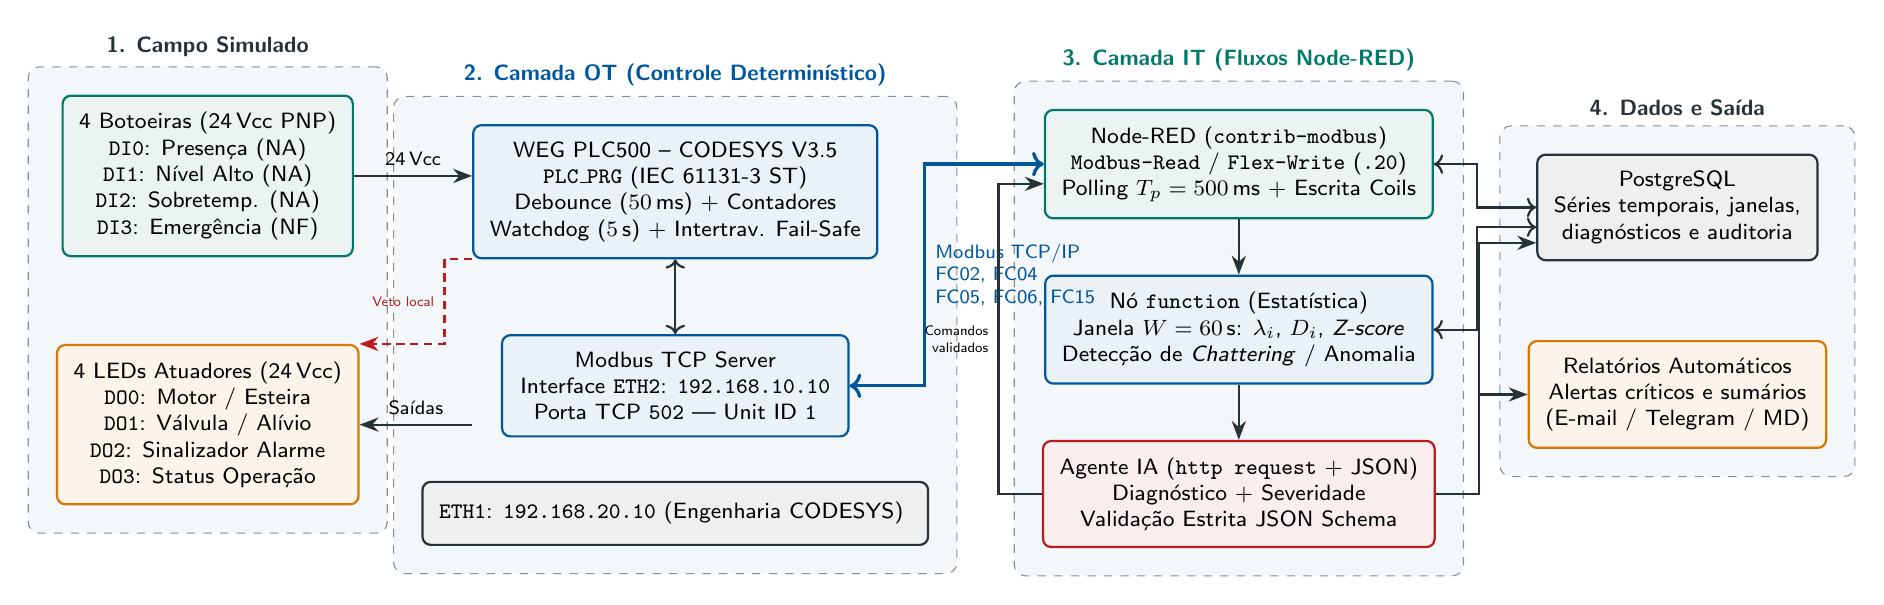
\begin{tikzpicture}[
    node distance=0.8cm and 1.1cm,
    font=\sffamily\footnotesize,
    box/.style={
      rectangle, rounded corners=3pt, draw=#1, fill=#1!8,
      thick, align=center, minimum height=1.15cm, inner sep=6pt
    },
    layer/.style={
      rectangle, rounded corners=4pt, draw=slateink!55, dashed,
      fill=steelbg, inner sep=10pt
    },
    arr/.style={-{Stealth[length=2.4mm]}, thick, draw=slateink},
    mbarr/.style={-{Stealth[length=2.4mm]}, very thick, draw=wegblue},
    safe/.style={-{Stealth[length=2.4mm]}, thick, draw=crimsonalert, densely dashed}
  ]

    % --- Camada de Campo ---
    \node[box=tealnode, minimum width=3.6cm] (botoeiras) {%
      \textbf{4 Botoeiras (24\,Vcc PNP)}\\
      \texttt{DI0}: Presença (NA)\\
      \texttt{DI1}: Nível Alto (NA)\\
      \texttt{DI2}: Sobretemp. (NA)\\
      \texttt{DI3}: Emergência (\textbf{NF})
    };
    \node[box=amberwarn, minimum width=3.6cm, below=1.1cm of botoeiras] (leds) {%
      \textbf{4 LEDs Atuadores (24\,Vcc)}\\
      \texttt{DO0}: Motor / Esteira\\
      \texttt{DO1}: Válvula / Alívio\\
      \texttt{DO2}: Sinalizador Alarme\\
      \texttt{DO3}: Status Operação
    };

    % --- Camada OT: WEG PLC500 ---
    \node[box=wegblue, minimum width=4.4cm, right=1.5cm of botoeiras, yshift=-0.2cm] (plcprg) {%
      \textbf{WEG PLC500 -- CODESYS V3.5}\\
      \texttt{PLC\_PRG} (IEC 61131-3 ST)\\
      Debounce ($50\,\text{ms}$) + Contadores\\
      Watchdog ($5\,\text{s}$) + \textbf{Intertrav. Fail-Safe}
    };
    \node[box=wegblue, minimum width=4.4cm, below=0.95cm of plcprg] (mbsrv) {%
      \textbf{Modbus TCP Server}\\
      Interface \texttt{ETH2}: \texttt{192.168.10.10}\\
      Porta TCP \texttt{502} | Unit ID \texttt{1}
    };
    \node[box=slateink, minimum width=4.4cm, below=0.55cm of mbsrv, minimum height=0.8cm] (eth1) {%
      \texttt{ETH1}: \texttt{192.168.20.10} (Engenharia CODESYS)
    };

    % --- Camada IT: Node-RED + IA + PostgreSQL ---
    \node[box=tealnode, minimum width=4.3cm, right=2.1cm of plcprg, yshift=0.35cm] (nrmb) {%
      \textbf{Node-RED (\texttt{contrib-modbus})}\\
      \texttt{Modbus-Read} / \texttt{Flex-Write} (\texttt{.20})\\
      Polling $T_p=500\,\text{ms}$ + Escrita Coils
    };
    \node[box=wegblue, minimum width=4.3cm, below=0.7cm of nrmb] (stats) {%
      \textbf{Nó \texttt{function} (Estatística)}\\
      Janela $W=60\,\text{s}$: $\lambda_i$, $D_i$, \textit{Z-score}\\
      Detecção de \textit{Chattering} / Anomalia
    };
    \node[box=crimsonalert, minimum width=4.3cm, below=0.7cm of stats] (llm) {%
      \textbf{Agente IA (\texttt{http request} + JSON)}\\
      Diagnóstico + Severidade\\
      \textbf{Validação Estrita JSON Schema}
    };

    % --- Persistência e Relatórios ---
    \node[box=slateink, minimum width=3.5cm, right=1.3cm of nrmb, yshift=-0.55cm] (pg) {%
      \textbf{PostgreSQL}\\
      Séries temporais, janelas,\\
      diagnósticos e auditoria
    };
    \node[box=amberwarn, minimum width=3.5cm, below=1.0cm of pg] (rep) {%
      \textbf{Relatórios Automáticos}\\
      Alertas críticos e sumários\\
      (E-mail / Telegram / MD)
    };

    % --- Agrupadores de camada ---
    \begin{scope}[on background layer]
      \node[layer, fit=(botoeiras)(leds), label={[font=\sffamily\bfseries\footnotesize, text=slateink]above:1. Campo Simulado}] (gcampo) {};
      \node[layer, fit=(plcprg)(mbsrv)(eth1), label={[font=\sffamily\bfseries\footnotesize, text=wegblue]above:2. Camada OT (Controle Determinístico)}] (got) {};
      \node[layer, fit=(nrmb)(stats)(llm), label={[font=\sffamily\bfseries\footnotesize, text=tealnode]above:3. Camada IT (Fluxos Node-RED)}] (git) {};
      \node[layer, fit=(pg)(rep), label={[font=\sffamily\bfseries\footnotesize, text=slateink]above:4. Dados e Saída}] (gout) {};
    \end{scope}

    % --- Conexões ---
    \draw[arr] (botoeiras.east) -- node[above, font=\sffamily\scriptsize]{24\,Vcc} (plcprg.west |- botoeiras.east);
    \draw[arr] (plcprg.west |- leds.east) -- node[above, font=\sffamily\scriptsize]{Saídas} (leds.east);
    \draw[safe] (plcprg.south west) -- ++(-0.35,0) |- node[pos=0.25, left, font=\sffamily\tiny, text=crimsonalert]{Veto local} (leds.north east);
    \draw[arr, <->] (plcprg.south) -- (mbsrv.north);

    \draw[mbarr, <->] (mbsrv.east) -- ++(0.95,0) |- node[pos=0.25, right, font=\sffamily\scriptsize, align=left, text=wegblue]{Modbus TCP/IP\\FC02, FC04\\FC05, FC06, FC15} (nrmb.west);

    \draw[arr] (nrmb.south) -- (stats.north);
    \draw[arr] (stats.south) -- (llm.north);
    \draw[arr] (llm.west) -- ++(-0.55,0) |- node[pos=0.25, left, font=\sffamily\tiny, align=right]{Comandos\\validados} ([yshift=-0.25cm]nrmb.west);

    \draw[arr, <->] (nrmb.east) -- ++(0.55,0) |- (pg.west);
    \draw[arr, <->] (stats.east) -- ++(0.55,0) |- ([yshift=-0.25cm]pg.west);
    \draw[arr] (llm.east) -- ++(0.55,0) |- ([yshift=-0.45cm]pg.west);
    \draw[arr] (llm.east) -- ++(0.55,0) |- (rep.west);
  \end{tikzpicture}%
  }
  \fonte{Elaborado pelos autores (2026).}
\end{figure}

\section{Especificação da Camada de Campo Simulada (Botoeiras e LEDs)}
\label{sec:arq_campo}

Para simular um subsistema industrial de transporte e controle de fluido sujeito a distúrbios operacionais, utilizam-se quatro das oito entradas digitais nativas e quatro das oito saídas digitais nativas de 24\,Vcc PNP do WEG PLC500, mantendo metade dos canais físicos como reserva para expansões futuras. No monorrepo do projeto, a documentação executiva completa dessa bancada encontra-se formalizada na lista de materiais \texttt{hardware/\allowbreak bom.csv}, na tabela de fiação \texttt{hardware/\allowbreak wiring\_\allowbreak table.md}, nos diagramas vetoriais CircuiTikZ/TikZ (\texttt{hardware/\allowbreak latex/\allowbreak schematic\_\allowbreak electrical.tex} e \texttt{schematic\_\allowbreak network\_\allowbreak bench.tex}, compilados em PDF, SVG e PNG de $300\,\text{DPI}$ em \texttt{hardware/\allowbreak diagrams/}) e no projeto eletrônico nativo do KiCad~8 (\texttt{hardware/\allowbreak kicad/\allowbreak plc500\_\allowbreak bench.kicad\_\allowbreak pro} e esquemático S-expression \texttt{plc500\_\allowbreak bench.kicad\_\allowbreak sch}).

A Tabela~\ref{tab:mapeamento_io} especifica a função de cada canal, o tipo de contato elétrico, o endereço IEC 61131-3 e o papel no processo simulado. A entrada \texttt{DI3} (\texttt{B4\_Emergencia}) utiliza obrigatoriamente contato \textbf{Normalmente Fechado (NF)}: em operação normal, o borne recebe $+24\,\text{Vcc}$ (\texttt{TRUE}); tanto o pressionamento do botão quanto eventual rompimento do cabo derrubam o sinal para $0\,\text{Vcc}$ (\texttt{FALSE}), levando o CLP imediatamente ao estado de bloqueio seguro (\textit{fail-safe}) \cite{moraes_castrucci}.

\begin{table}[htb]
  \centering
  \SingleSpacing
  \caption{Mapeamento das entradas (botoeiras) e saídas digitais (LEDs) nativas do WEG PLC500}
  \label{tab:mapeamento_io}
  \footnotesize
  \begin{tabularx}{\textwidth}{@{}p{1.05cm}p{1.2cm}p{3.0cm}p{1.25cm}p{1.7cm}L@{}}
    \toprule
    \textbf{Canal} & \textbf{IEC} & \textbf{Identificador} & \textbf{Tipo} & \textbf{Elemento} & \textbf{Semântica Industrial Simulada} \\
    \midrule
    \texttt{DI0} & \texttt{\%IX0.0} & \texttt{B1\_SensPresenca} & NA (PNP) & Botoeira 1 & Sensor óptico/indutivo de passagem de peça na esteira (eventos de ciclo) \\
    \texttt{DI1} & \texttt{\%IX0.1} & \texttt{B2\_SensNivelAlto} & NA (PNP) & Botoeira 2 & Chave de nível máximo de reservatório (indica risco de transbordamento) \\
    \texttt{DI2} & \texttt{\%IX0.2} & \texttt{B3\_SensSobretemp} & NA (PNP) & Botoeira 3 & Termostato digital de sobretemperatura no conjunto motor-bomba \\
    \texttt{DI3} & \texttt{\%IX0.3} & \texttt{B4\_Emergencia} & \textbf{NF} (PNP) & Botoeira 4 & Parada de emergência com lógica \textit{fail-safe} (\texttt{FALSE} = emergência ativa) \\
    \midrule
    \texttt{DO0} & \texttt{\%QX0.0} & \texttt{L1\_AtuMotor} & PNP 24\,V & LED Verde & Comando do motor/esteira principal (desligado em falha crítica/emergência) \\
    \texttt{DO1} & \texttt{\%QX0.1} & \texttt{L2\_AtuValvula} & PNP 24\,V & LED Amarelo & Acionamento de válvula solenoide ou bomba auxiliar de alívio/resfriamento \\
    \texttt{DO2} & \texttt{\%QX0.2} & \texttt{L3\_SinalAlarme} & PNP 24\,V & LED Vermelho & Sinalizador óptico/sonoro de anomalia crítica, watchdog ou emergência \\
    \texttt{DO3} & \texttt{\%QX0.3} & \texttt{L4\_StatusOper} & PNP 24\,V & LED Branco & Indicador de operação normal com enlace Modbus TCP/IP saudável \\
    \bottomrule
  \end{tabularx}
  \fonte{Elaborado pelos autores (2026).}
\end{table}

Cada saída digital PNP de 24\,Vcc aciona um sinaleiro LED industrial de 24\,Vcc (ou LED discreto em série com resistor limitador de filme metálico de $2{,}2\,\text{k}\Omega$ / $0{,}5\,\text{W}$, dentro da faixa nominal de $1{,}8\,\text{k}\Omega$ a $2{,}2\,\text{k}\Omega$), resultando em corrente nominal de aproximadamente $10\,\text{mA}$ por canal.

\section{Mapa de Registradores Modbus TCP/IP}
\label{sec:arq_modbus}

O contrato de memória entre o WEG PLC500 (\textit{Modbus TCP Server}) e o Node-RED (\textit{Modbus TCP Client}) segrega variáveis de leitura (\textit{Discrete Inputs} e \textit{Input Registers}) e variáveis de escrita supervisória (\textit{Coils} e \textit{Holding Registers}), adotando endereçamento base zero (\textit{0-based}) na PDU \cite{modbus_app_v11b3}. Esse contrato de 23 registradores é exportado de forma canônica em \texttt{plc/codesys/modbus\_mapping.csv} em paridade estrita com a lista de variáveis globais \texttt{plc/src/GVL\_Modbus.st}. A Tabela~\ref{tab:mapa_modbus} apresenta o mapeamento completo.

\begin{table}[htb]
  \centering
  \SingleSpacing
  \caption{Mapa completo de registradores Modbus TCP/IP expostos pelo WEG PLC500 (Unit ID 1, porta 502)}
  \label{tab:mapa_modbus}
  \scriptsize
  \begin{tabularx}{\textwidth}{@{}>{\RaggedRight\arraybackslash}p{2.15cm}p{0.80cm}p{1.15cm}p{3.40cm}L@{}}
    \toprule
    \textbf{Área Modbus} & \textbf{End.} & \textbf{FC} & \textbf{Variável PLC500} & \textbf{Descrição Funcional e Faixa de Valores} \\
    \midrule
    \multirow{6}{2.15cm}{\RaggedRight\textit{Discrete Inputs} (Leitura, 1 bit)}
      & \texttt{0} & \texttt{FC02} & \texttt{xDI\_Presenca} & Estado filtrado (\textit{debounce}) de \texttt{B1\_SensPresenca} \\
      & \texttt{1} & \texttt{FC02} & \texttt{xDI\_NivelAlto} & Estado filtrado de \texttt{B2\_SensNivelAlto} \\
      & \texttt{2} & \texttt{FC02} & \texttt{xDI\_Sobretemp} & Estado filtrado de \texttt{B3\_SensSobretemp} \\
      & \texttt{3} & \texttt{FC02} & \texttt{xDI\_EmergenciaOK} & Estado físico NF de \texttt{B4\_Emergencia} (\texttt{0} = atuada/fio partido) \\
      & \texttt{4} & \texttt{FC02} & \texttt{xFlag\_EmergTravada} & \texttt{1} se emergência travada aguardando rearme seguro \\
      & \texttt{5} & \texttt{FC02} & \texttt{xFlag\_WatchdogAtivo} & \texttt{1} se \textit{heartbeat} do Node-RED expirou ($> T_{wd}$) \\
    \midrule
    \multirow{5}{2.15cm}{\RaggedRight\textit{Coils} (Leitura e Escrita, 1 bit)}
      & \texttt{0} & \texttt{FC01/05} & \texttt{xCmd\_Motor} & Comando supervisório do Node-RED para \texttt{L1\_AtuMotor} \\
      & \texttt{1} & \texttt{FC01/05} & \texttt{xCmd\_Valvula} & Comando supervisório do Node-RED para \texttt{L2\_AtuValvula} \\
      & \texttt{2} & \texttt{FC01/05} & \texttt{xCmd\_Alarme} & Comando supervisório do Node-RED para \texttt{L3\_SinalAlarme} \\
      & \texttt{3} & \texttt{FC01/05} & \texttt{xCmd\_ResetFalha} & Pulso de rearme de falha (válido somente se \texttt{DI3=1} e \texttt{DI2=0}) \\
      & \texttt{4} & \texttt{FC01/05} & \texttt{xCmd\_HabRemoto} & Habilita modo automático supervisionado pelo Node-RED (\texttt{1} = ativo) \\
    \midrule
    \multirow{8}{2.15cm}{\RaggedRight\textit{Input Registers} (Leitura, 16 bits)}
      & \texttt{0} & \texttt{FC04} & \texttt{uiCnt\_Presenca} & Contador acumulado de bordas de subida de \texttt{B1} (0--65535) \\
      & \texttt{1} & \texttt{FC04} & \texttt{uiCnt\_NivelAlto} & Contador acumulado de acionamentos de \texttt{B2} (0--65535) \\
      & \texttt{2} & \texttt{FC04} & \texttt{uiCnt\_Sobretemp} & Contador acumulado de acionamentos de \texttt{B3} (0--65535) \\
      & \texttt{3} & \texttt{FC04} & \texttt{uiCnt\_Emergencia} & Contador acumulado de eventos de emergência em \texttt{B4} \\
      & \texttt{4} & \texttt{FC04} & \texttt{uiEstado\_CLP} & Código da máquina de estados: \texttt{0}=INIT, \texttt{1}=AUTO, \texttt{2}=ALERTA, \texttt{3}=DEGRADADO, \texttt{4}=EMERG \\
      & \texttt{5} & \texttt{FC04} & \texttt{wMascara\_DO\_Real} & Bitmask das saídas físicas reais (\texttt{bit0=DO0}..\texttt{bit3=DO3}) \\
      & \texttt{6} & \texttt{FC04} & \texttt{uiEcho\_Heartbeat} & Eco do último valor de \textit{heartbeat} recebido do Node-RED \\
      & \texttt{7} & \texttt{FC04} & \texttt{uiCod\_Intertrav} & Causa de veto local: \texttt{0}=Nenhum, \texttt{1}=Emerg., \texttt{2}=Sobretemp., \texttt{3}=Watchdog \\
    \midrule
    \multirow{4}{2.15cm}{\RaggedRight\textit{Holding Registers} (Leitura e Escrita, 16 bits)}
      & \texttt{0} & \texttt{FC03/06} & \texttt{uiHeartbeat\_NR} & Contador cíclico (1--65535) incrementado pelo Node-RED (alias \texttt{uiHeartbeat\_Sup}) \\
      & \texttt{1} & \texttt{FC03/06} & \texttt{uiTimeout\_WD\_ms} & Limiar configurável do \textit{watchdog} em ms (padrão: \texttt{5000}) \\
      & \texttt{2} & \texttt{FC03/06} & \texttt{uiSeveridade\_IA} & Severidade reportada pela pipeline: \texttt{0}=NORMAL, \texttt{1}=ATENCAO, \texttt{2}=CRITICO, \texttt{3}=EMERG \\
      & \texttt{3} & \texttt{FC03/06} & \texttt{uiVersao\_Mapa} & Identificador de versão do contrato de mapa (valor fixo \texttt{100} = v1.0) \\
    \bottomrule
  \end{tabularx}
  \fonte{Elaborado pelos autores (2026).}
\end{table}

A leitura combinada de \texttt{wMascara\_DO\_Real} (\textit{Input Register}~\texttt{5}) e \texttt{uiCod\_Intertrav} (\textit{Input Register}~\texttt{7}) permite ao Node-RED auditar em malha fechada se o comando enviado aos \textit{Coils} foi efetivamente aplicado aos LEDs físicos ou se sofreu veto legítimo pelo intertravamento local do CLP.

\section{Dinâmica de Comunicação, Polling e Supervisão de Enlace}
\label{sec:arq_sequencia}

O fluxo no Node-RED opera com ciclo nominal de varredura $T_p = 500\,\text{ms}$. Em cada ciclo, os nós de leitura do \texttt{node-red-contrib-modbus} requisitam em bloco os 6 \textit{Discrete Inputs} (\texttt{FC02}) e os 8 \textit{Input Registers} (\texttt{FC04}), reduzindo o número de pacotes TCP e assegurando consistência entre estados instantâneos e contadores. Na sequência imediata, um nó \texttt{Modbus-Flex-Write} incrementa o \textit{Holding Register}~\texttt{0} (\texttt{uiHeartbeat\_NR}) via \texttt{FC06}.

Sempre que a análise estatística ou o diagnóstico validado do agente LLM solicita mudança nos atuadores, o Node-RED envia uma escrita múltipla de \textit{Coils} (\texttt{FC15}) e atualiza o nível de severidade em \texttt{uiSeveridade\_IA} (\texttt{FC06}). Caso ocorra desconexão Ethernet ou parada do serviço Node-RED, o temporizador interno do PLC500 identifica a ausência de incremento em \texttt{uiHeartbeat\_NR} após $T_{wd} = 5000\,\text{ms}$ e comuta para o estado seguro degradado, conforme ilustrado na Figura~\ref{fig:sequencia-modbus}.

\begin{figure}[htb]
  \centering
  \caption{Diagrama de sequência da comunicação Modbus TCP/IP entre WEG PLC500 e Node-RED}
  \label{fig:sequencia-modbus}
  \resizebox{\textwidth}{!}{%
  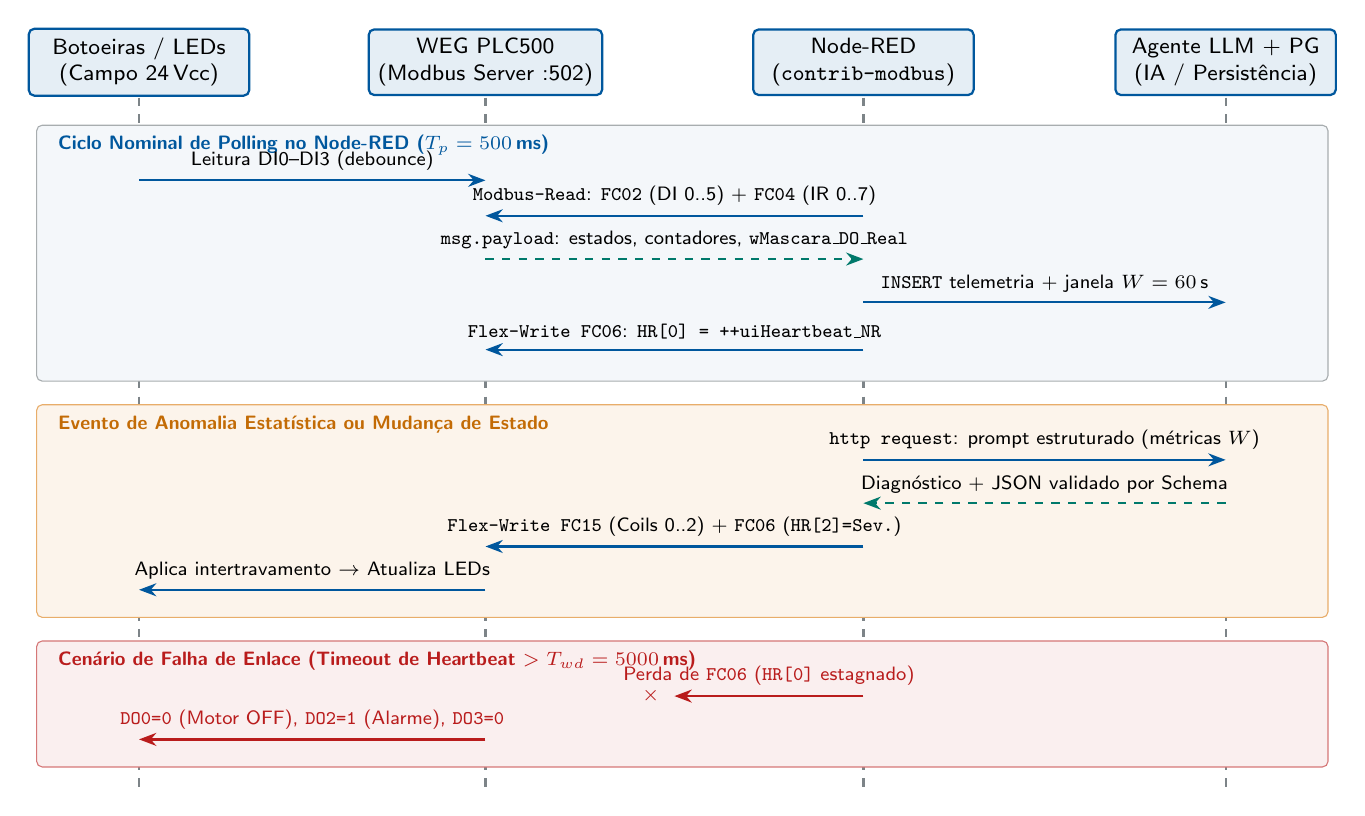
\begin{tikzpicture}[
    font=\sffamily\footnotesize,
    actor/.style={rectangle, rounded corners=2pt, draw=wegblue, fill=wegblue!10, thick, minimum width=2.8cm, minimum height=0.8cm, align=center},
    lifeline/.style={draw=slateink!60, dashed, thick},
    msg/.style={-{Stealth[length=2.2mm]}, thick, draw=wegblue},
    ret/.style={-{Stealth[length=2.2mm]}, thick, draw=tealnode, dashed},
    err/.style={-{Stealth[length=2.2mm]}, thick, draw=crimsonalert, thick}
  ]
    % Atores
    \node[actor] (a1) at (0,0) {\textbf{Botoeiras / LEDs}\\(Campo 24\,Vcc)};
    \node[actor] (a2) at (4.4,0) {\textbf{WEG PLC500}\\(Modbus Server :502)};
    \node[actor] (a3) at (9.2,0) {\textbf{Node-RED}\\(\texttt{contrib-modbus})};
    \node[actor] (a4) at (13.8,0) {\textbf{Agente LLM + PG}\\(IA / Persistência)};

    % Linhas de vida
    \foreach \x in {0, 4.4, 9.2, 13.8} {
      \draw[lifeline] (\x,-0.45) -- (\x,-9.2);
    }

    % Fase 1: Ciclo Nominal de Polling
    \draw[fill=steelbg, draw=slateink!40, rounded corners=2pt] (-1.3,-0.8) rectangle (15.1,-4.05);
    \node[anchor=west, font=\sffamily\bfseries\scriptsize, text=wegblue] at (-1.15,-1.05) {Ciclo Nominal de Polling no Node-RED ($T_p = 500\,\text{ms}$)};

    \draw[msg] (0,-1.5) -- node[above, font=\sffamily\scriptsize]{Leitura DI0--DI3 (debounce)} (4.4,-1.5);
    \draw[msg] (9.2,-1.95) -- node[above, font=\sffamily\scriptsize]{\texttt{Modbus-Read}: \texttt{FC02} (DI 0..5) + \texttt{FC04} (IR 0..7)} (4.4,-1.95);
    \draw[ret] (4.4,-2.5) -- node[above, font=\sffamily\scriptsize]{\texttt{msg.payload}: estados, contadores, \texttt{wMascara\_DO\_Real}} (9.2,-2.5);
    \draw[msg] (9.2,-3.05) -- node[above, font=\sffamily\scriptsize]{\texttt{INSERT} telemetria + janela $W=60\,\text{s}$} (13.8,-3.05);
    \draw[msg] (9.2,-3.65) -- node[above, font=\sffamily\scriptsize]{\texttt{Flex-Write FC06}: \texttt{HR[0] = ++uiHeartbeat\_NR}} (4.4,-3.65);

    % Fase 2: Detecção de Anomalia e Atuação Validada
    \draw[fill=amberwarn!8, draw=amberwarn!60, rounded corners=2pt] (-1.3,-4.35) rectangle (15.1,-7.05);
    \node[anchor=west, font=\sffamily\bfseries\scriptsize, text=amberwarn!90!black] at (-1.15,-4.6) {Evento de Anomalia Estatística ou Mudança de Estado};

    \draw[msg] (9.2,-5.05) -- node[above, font=\sffamily\scriptsize]{\texttt{http request}: prompt estruturado (métricas $W$)} (13.8,-5.05);
    \draw[ret] (13.8,-5.6) -- node[above, font=\sffamily\scriptsize]{Diagnóstico + JSON validado por Schema} (9.2,-5.6);
    \draw[msg] (9.2,-6.15) -- node[above, font=\sffamily\scriptsize]{\texttt{Flex-Write FC15} (Coils 0..2) + \texttt{FC06} (\texttt{HR[2]=Sev.})} (4.4,-6.15);
    \draw[msg] (4.4,-6.7) -- node[above, font=\sffamily\scriptsize]{Aplica intertravamento $\rightarrow$ Atualiza LEDs} (0,-6.7);

    % Fase 3: Perda de Comunicação / Watchdog
    \draw[fill=crimsonalert!7, draw=crimsonalert!60, rounded corners=2pt] (-1.3,-7.35) rectangle (15.1,-8.95);
    \node[anchor=west, font=\sffamily\bfseries\scriptsize, text=crimsonalert] at (-1.15,-7.6) {Cenário de Falha de Enlace (\textit{Timeout} de \textit{Heartbeat} $> T_{wd} = 5000\,\text{ms}$)};

    \draw[err] (9.2,-8.05) -- node[above, font=\sffamily\scriptsize, text=crimsonalert]{Perda de \texttt{FC06} (\texttt{HR[0]} estagnado)} (6.8,-8.05);
    \node[font=\sffamily\bfseries\scriptsize, text=crimsonalert] at (6.5,-8.05) {$\times$};
    \draw[err] (4.4,-8.6) -- node[above, font=\sffamily\scriptsize, text=crimsonalert]{\texttt{DO0=0} (Motor OFF), \texttt{DO2=1} (Alarme), \texttt{DO3=0}} (0,-8.6);
  \end{tikzpicture}%
  }
  \fonte{Elaborado pelos autores (2026).}
\end{figure}

% ==============================================================================
% capitulos/04_implementacao_clp.tex
% Capítulo 4 — Implementação da Camada de Controle (WEG PLC500 / CODESYS)
% Inclui Diagrama TikZ 3 (Máquina de Estados) e Quadro 1 (Código IEC 61131-3 ST)
% ==============================================================================

\chapter{Implementação da Camada de Controle (WEG PLC500 / CODESYS)}
\label{cap:implementacao_clp}

Este capítulo especifica a configuração do servidor Modbus TCP/IP no ambiente CODESYS V3.5 para o controlador WEG PLC500, o modelo comportamental em máquina de estados finitos e a implementação de referência da lógica determinística de aquisição, filtragem, supervisão de enlace e intertravamento \textit{fail-safe} em linguagem \textit{Structured Text} (IEC 61131-3).

\section{Configuração no Ambiente CODESYS V3.5}
\label{sec:clp_codesys}

Conforme a nota de aplicação oficial da WEG para comunicação Modbus TCP no PLC500 \cite{weg_plc500_modbus} e a documentação do ambiente CODESYS V3.5 \cite{codesys_v35}, a exposição das tabelas de memória na interface \texttt{ETH2} requer a estruturação hierárquica da árvore de dispositivos (\textit{Device Tree}) na seguinte ordem:

\begin{enumerate}
  \item \textbf{Dispositivo Raiz (\texttt{Device -- WEG PLC500}):} configura a tarefa cíclica principal (\texttt{MainTask}) com período determinístico de varredura de $10\,\text{ms}$ e prioridade alta para execução do programa \texttt{PLC\_PRG}.
  \item \textbf{Adaptador Ethernet (\texttt{Ethernet\_ETH2}):} associado à porta física \texttt{ETH2} do PLC500 com endereço IP estático \texttt{192.168.10.10} e máscara \texttt{255.255.255.0}.
  \item \textbf{Dispositivo Servidor Modbus (\texttt{ModbusTCP\_Server\_Device}):} inserido como filho de \texttt{Ethernet\_ETH2}, configurado com porta TCP \texttt{502}, \textit{Unit ID} \texttt{1}, máximo de 4 conexões simultâneas e tempo limite de inatividade de \textit{socket} de $10\,\text{s}$.
  \item \textbf{Mapeamento de Canais (\textit{Modbus Server I/O Mapping}):} vincula os endereços base zero definidos na Tabela~\ref{tab:mapa_modbus} às variáveis globais de interface (\textit{Discrete Inputs} \texttt{0..5}, \textit{Coils} \texttt{0..4}, \textit{Input Registers} \texttt{0..7} e \textit{Holding Registers} \texttt{0..3}), ativando a opção de atualização contínua de variáveis em cada ciclo da tarefa principal.
\end{enumerate}

As entradas e saídas digitais nativas do PLC500 são mapeadas na seção \textit{Local\_IO} do projeto CODESYS diretamente para os endereços físicos \texttt{\%IX0.0} a \texttt{\%IX0.3} (botoeiras) e \texttt{\%QX0.0} a \texttt{\%QX0.3} (LEDs).

\section{Filtragem de Entradas, Watchdog e Intertravamento de Segurança}
\label{sec:clp_seguranca}

O software embarcado no CLP concentra todas as decisões críticas de segurança e integridade de sinal, garantindo que imperfeições eletromecânicas ou falhas da camada IT não comprometam o processo:

\begin{itemize}
  \item \textbf{Filtro de \textit{debounce} digital ($T_{db} = 50\,\text{ms}$):} contatos mecânicos de botoeiras apresentam repique transitório durante a comutação. Cada entrada de processo (\texttt{DI0}--\texttt{DI2}) passa por um temporizador com retardo na energização (\texttt{TON}) de $50\,\text{ms}$ antes de atualizar o sinal filtrado e incrementar seu respectivo contador de borda (\texttt{R\_TRIG}). A entrada de parada de emergência (\texttt{DI3}, contato NF) atua \textbf{sem retardo de energização}, garantindo interrupção imediata no primeiro ciclo de varredura em que o contato abrir.
  \item \textbf{Supervisão de \textit{heartbeat} (\textit{watchdog}):} a cada ciclo, o CLP compara o registrador \texttt{uiHeartbeat\_NR} com o valor armazenado no ciclo anterior. Enquanto houver mudança, um temporizador \texttt{TON} (\texttt{tonWatchdog}) é reiniciado e o valor é ecoado em \texttt{uiEcho\_Heartbeat}. Se o registrador permanecer inalterado por tempo superior a $T_{wd}$ (padrão $5000\,\text{ms}$, ajustável entre $2000\,\text{ms}$ e $30000\,\text{ms}$), ativa-se \texttt{xFlag\_WatchdogAtivo}.
  \item \textbf{Hierarquia estrita de precedência de atuação:} a atribuição final das saídas físicas (\texttt{DO0}--\texttt{DO3}) obedece à prioridade decrescente: (1)~Parada de Emergência Travada (\texttt{EMERGENCIA\_TRAVADA}); (2)~Intertravamento local por Sobretemperatura (\texttt{xDI\_Sobretemp}); (3)~Modo Degradado por \textit{Watchdog} (\texttt{MODO\_DEGRADADO\_WD}); (4)~Comandos supervisórios recebidos do Node-RED via Modbus TCP/IP quando \texttt{xCmd\_HabRemoto = TRUE}.
\end{itemize}

\section{Máquina de Estados Finitos do Controlador}
\label{sec:clp_estados}

Para tornar o comportamento do WEG PLC500 plenamente previsível e auditável pela pipeline analítica no Node-RED, o estado operacional é modelado pela máquina de estados finitos apresentada na Figura~\ref{fig:maquina-estados-clp}. O identificador numérico do estado atual é publicado continuamente no \textit{Input Register}~\texttt{4} (\texttt{uiEstado\_CLP}).

\begin{figure}[htb]
  \centering
  \caption{Máquina de estados finitos e regras de intertravamento determinístico no WEG PLC500}
  \label{fig:maquina-estados-clp}
  \resizebox{\textwidth}{!}{%
  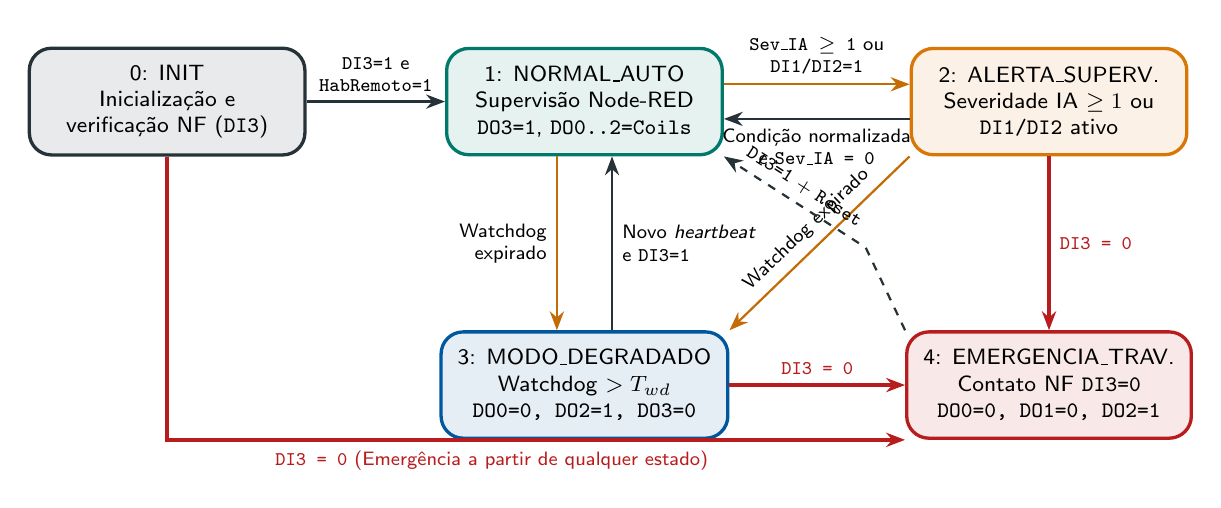
\begin{tikzpicture}[
    font=\sffamily\footnotesize,
    state/.style={
      rectangle, rounded corners=8pt, draw=#1, fill=#1!10,
      very thick, minimum width=3.5cm, minimum height=1.35cm, align=center, inner sep=6pt
    },
    trans/.style={-{Stealth[length=2.4mm]}, thick, draw=slateink},
    crit/.style={-{Stealth[length=2.4mm]}, very thick, draw=crimsonalert},
    warn/.style={-{Stealth[length=2.4mm]}, thick, draw=amberwarn!90!black}
  ]

    \node[state=slateink] (init) at (0,0) {\textbf{0: INIT}\\Inicialização e\\verificação NF (\texttt{DI3})};
    \node[state=tealnode] (auto) at (5.3,0) {\textbf{1: NORMAL\_AUTO}\\Supervisão Node-RED\\\texttt{DO3=1}, \texttt{DO0..2=Coils}};
    \node[state=amberwarn] (alerta) at (11.2,0) {\textbf{2: ALERTA\_SUPERV.}\\Severidade IA $\ge 1$ ou\\\texttt{DI1/DI2} ativo};
    \node[state=wegblue] (deg) at (5.3,-3.6) {\textbf{3: MODO\_DEGRADADO}\\Watchdog $> T_{wd}$\\\texttt{DO0=0, DO2=1, DO3=0}};
    \node[state=crimsonalert] (emerg) at (11.2,-3.6) {\textbf{4: EMERGENCIA\_TRAV.}\\Contato NF \texttt{DI3=0}\\\texttt{DO0=0, DO1=0, DO2=1}};

    % Transições nominais
    \draw[trans] (init.east) -- node[above, font=\sffamily\scriptsize, align=center]{\texttt{DI3=1} e\\\texttt{HabRemoto=1}} (auto.west);
    \draw[warn] ([yshift=0.22cm]auto.east) -- node[above, font=\sffamily\scriptsize, align=center]{\texttt{Sev\_IA $\ge$ 1} ou\\\texttt{DI1/DI2=1}} ([yshift=0.22cm]alerta.west);
    \draw[trans] ([yshift=-0.22cm]alerta.west) -- node[below, font=\sffamily\scriptsize, align=center]{Condição normalizada\\e \texttt{Sev\_IA = 0}} ([yshift=-0.22cm]auto.east);

    % Transições de Watchdog
    \draw[warn] ([xshift=-0.35cm]auto.south) -- node[left, font=\sffamily\scriptsize, align=right]{Watchdog\\expirado} ([xshift=-0.35cm]deg.north);
    \draw[trans] ([xshift=0.35cm]deg.north) -- node[right, font=\sffamily\scriptsize, align=left]{Novo \textit{heartbeat}\\e \texttt{DI3=1}} ([xshift=0.35cm]auto.south);
    \draw[warn] (alerta.south west) -- node[above, sloped, font=\sffamily\scriptsize]{Watchdog expirado} (deg.north east);

    % Transições de Emergência (precedência máxima)
    \draw[crit] (init.south) |- node[pos=0.72, below, font=\sffamily\scriptsize, text=crimsonalert]{\texttt{DI3 = 0} (Emergência a partir de qualquer estado)} (emerg.south west);
    \draw[crit] (alerta.south) -- node[right, font=\sffamily\scriptsize, text=crimsonalert]{\texttt{DI3 = 0}} (emerg.north);
    \draw[crit] (deg.east) -- node[above, font=\sffamily\scriptsize, text=crimsonalert]{\texttt{DI3 = 0}} (emerg.west);
    \draw[trans, dashed] (emerg.north west) -- ++(-0.5,1.05) -- node[above, sloped, font=\sffamily\scriptsize]{\texttt{DI3=1} + \texttt{Reset}} (auto.south east);
  \end{tikzpicture}%
  }
  \fonte{Elaborado pelos autores (2026).}
\end{figure}

\section{Implementação em Structured Text (IEC 61131-3)}
\label{sec:clp_codigo}

No repositório do projeto, o firmware IEC 61131-3 é estruturado de forma modular no diretório \texttt{plc/src/} em cinco unidades de organização de programa (POUs) reutilizáveis: (i)~\texttt{GVL\_Modbus.st}, lista de variáveis globais qualificada com \texttt{\{attribute 'qualified\_only'\}} contendo os 23 pontos do contrato Modbus TCP/IP (em que \texttt{HR[0]} é declarado como \texttt{uiHeartbeat\_Sup}, mantendo \texttt{uiHeartbeat\_NR} como alias de compatibilidade documentado); (ii)~\texttt{FB\_DebounceCounter.st}, bloco funcional que encapsula o temporizador \texttt{TON} de $50\,\text{ms}$, o detector de borda \texttt{R\_TRIG} e o contador modular de 16~bits; (iii)~\texttt{FB\_WatchdogHeartbeat.st}, responsável pela validação de limites $[2000, 30000]\,\text{ms}$ (com \textit{fallback} seguro para \texttt{T\#5S}), avaliação de \texttt{tonWatchdog} previamente à atualização de \texttt{uiLastHeartbeat} e cópia para \texttt{uiEcho\_Heartbeat}; (iv)~\texttt{FB\_SafetyInterlock.st}, que implementa a máquina de estados, o rearme por borda de subida e a hierarquia estrita de intertravamento; e (v)~\texttt{PLC\_PRG.st}, programa principal associado à tarefa cíclica \texttt{MainTask} ($10\,\text{ms}$). Adicionalmente, o pacote \texttt{plc/codesys/} disponibiliza o projeto completo no padrão aberto \textbf{PLCopen TC6 XML v2.01} (\texttt{plc500\_project\_plcopen.xml}) para importação direta no CODESYS V3.5 e a tabela de vinculação base zero \texttt{modbus\_mapping.csv}.

O Quadro~\ref{quadro:codigo_st} apresenta a lógica consolidada equivalente de \texttt{PLC\_PRG} em \textit{Structured Text} para o WEG PLC500. O código separa claramente leitura física filtrada, contadores acumulados de 16~bits, avaliação de \textit{watchdog} sobre o registrador \texttt{uiHeartbeat\_NR} (\texttt{uiHeartbeat\_Sup}), rearme seguro de emergência sensível à borda de subida (\texttt{rtReset.Q}), intertravamento local de sobretemperatura e composição da máscara de retorno \texttt{wMascara\_DO\_Real}.

\begin{quadro}[htb]
  \centering
  \SingleSpacing
  \caption{Implementação em Structured Text (IEC 61131-3) do programa \texttt{PLC\_PRG} no WEG PLC500}
  \label{quadro:codigo_st}
  \begin{lstlisting}[language=IECST, basicstyle=\linespread{0.85}\selectfont\ttfamily\tiny\color{black}]
PROGRAM PLC_PRG
VAR
  tonDebPresenca, tonDebNivel, tonDebTemp      : TON;
  rtPresenca, rtNivel, rtTemp, rtEmerg, rtReset : R_TRIG;
  tonWatchdog      : TON;
  uiLastHeartbeat  : UINT := 0;
  tWatchdogLimit   : TIME := T#5S;
END_VAR
// 1. Debounce das entradas de processo (DI0..DI2) e leitura imediata NF (DI3)
tonDebPresenca(IN := %IX0.0, PT := T#50MS);
tonDebNivel   (IN := %IX0.1, PT := T#50MS);
tonDebTemp    (IN := %IX0.2, PT := T#50MS);
xDI_Presenca     := tonDebPresenca.Q;
xDI_NivelAlto    := tonDebNivel.Q;
xDI_Sobretemp    := tonDebTemp.Q;
xDI_EmergenciaOK := %IX0.3; // Contato NF: FALSE = emergencia acionada
// 2. Contadores acumulados de eventos (Input Registers 0..3)
rtPresenca(CLK := xDI_Presenca);   IF rtPresenca.Q THEN uiCnt_Presenca  := uiCnt_Presenca + 1; END_IF;
rtNivel   (CLK := xDI_NivelAlto);  IF rtNivel.Q    THEN uiCnt_NivelAlto := uiCnt_NivelAlto + 1; END_IF;
rtTemp    (CLK := xDI_Sobretemp);  IF rtTemp.Q     THEN uiCnt_Sobretemp := uiCnt_Sobretemp + 1; END_IF;
rtEmerg   (CLK := NOT xDI_EmergenciaOK);
IF rtEmerg.Q THEN uiCnt_Emergencia := uiCnt_Emergencia + 1; END_IF;
// 3. Supervisao de enlace Modbus TCP/IP (Watchdog via Holding Register 0)
IF (uiTimeout_WD_ms >= 2000) AND (uiTimeout_WD_ms <= 30000) THEN
  tWatchdogLimit := UINT_TO_TIME(uiTimeout_WD_ms);
ELSE
  tWatchdogLimit := T#5S;
END_IF;
tonWatchdog(IN := (uiHeartbeat_NR = uiLastHeartbeat), PT := tWatchdogLimit);
IF uiHeartbeat_NR <> uiLastHeartbeat THEN
  uiLastHeartbeat  := uiHeartbeat_NR;
  uiEcho_Heartbeat := uiHeartbeat_NR;
END_IF;
xFlag_WatchdogAtivo := tonWatchdog.Q;
// 4. Travamento de emergencia (fail-safe) e rearme seguro por borda de subida
rtReset(CLK := xCmd_ResetFalha);
IF NOT xDI_EmergenciaOK THEN
  xFlag_EmergTravada := TRUE;
ELSIF xCmd_ResetFalha AND rtReset.Q AND xDI_EmergenciaOK AND (NOT xDI_Sobretemp) THEN
  xFlag_EmergTravada := FALSE;
END_IF;
// 5. Maquina de estados e intertravamento local com precedencia sobre o Node-RED
IF xFlag_EmergTravada THEN
  uiEstado_CLP := 4; uiCod_Intertrav := 1;
  %QX0.0 := FALSE; %QX0.1 := FALSE; %QX0.2 := TRUE;  %QX0.3 := FALSE;
ELSIF xDI_Sobretemp THEN
  uiEstado_CLP := 2; uiCod_Intertrav := 2; // Protecao termica local
  %QX0.0 := FALSE; %QX0.1 := TRUE;  %QX0.2 := TRUE;  %QX0.3 := (NOT xFlag_WatchdogAtivo) AND xCmd_HabRemoto;
ELSIF xFlag_WatchdogAtivo THEN
  uiEstado_CLP := 3; uiCod_Intertrav := 3; // Perda de comunicacao com Node-RED
  %QX0.0 := FALSE; %QX0.1 := xDI_NivelAlto; %QX0.2 := TRUE; %QX0.3 := FALSE;
ELSIF xCmd_HabRemoto THEN
  uiCod_Intertrav := 0;
  uiEstado_CLP := SEL((uiSeveridade_IA > 0) OR xDI_NivelAlto, 1, 2);
  %QX0.0 := xCmd_Motor;
  %QX0.1 := xCmd_Valvula OR xDI_NivelAlto; // Alivio garantido em nivel alto
  %QX0.2 := xCmd_Alarme OR (uiSeveridade_IA >= 2);
  %QX0.3 := TRUE;
ELSE
  // Estado INIT (xCmd_HabRemoto = FALSE): uiEstado_CLP := 0; uiCod_Intertrav := 0;
  uiEstado_CLP := 0; uiCod_Intertrav := 0;
  %QX0.0 := FALSE; %QX0.1 := FALSE; %QX0.2 := FALSE; %QX0.3 := FALSE;
END_IF;
// 6. Espelhamento das saidas fisicas reais em bitmask (Input Register 5)
wMascara_DO_Real := BOOL_TO_WORD(%QX0.0) OR SHL(BOOL_TO_WORD(%QX0.1), 1)
                 OR SHL(BOOL_TO_WORD(%QX0.2), 2) OR SHL(BOOL_TO_WORD(%QX0.3), 3);
uiVersao_Mapa := 100;
END_PROGRAM
  \end{lstlisting}
  \fonte{Elaborado pelos autores (2026).}
\end{quadro}

Observa-se na seção~5 do Quadro~\ref{quadro:codigo_st} que o LED indicador de operação normal (\texttt{\%QX0.3}) permanece aceso apenas quando não há emergência travada, o modo remoto está habilitado e o \textit{watchdog} está saudável. De modo análogo, o acionamento da válvula de alívio (\texttt{\%QX0.1}) combina o comando supervisório com o disparo local por nível alto (\texttt{xDI\_NivelAlto}) e por sobretemperatura (\texttt{xDI\_Sobretemp}), assegurando resposta determinística em até um ciclo de varredura ($10\,\text{ms}$).

% ==============================================================================
% capitulos/05_implementacao_nodered.tex
% Capítulo 5 — Implementação da Pipeline Analítica no Node-RED e Persistência
% Inclui Diagrama TikZ 4, Equações Estatísticas, Quadros 2, 3, 4 e 5
% ==============================================================================

\chapter{Implementação da Pipeline Analítica no Node-RED e Persistência}
\label{cap:implementacao_nodered}

Este capítulo detalha a camada de Tecnologia da Informação (IT) responsável pela coleta contínua de dados via Modbus TCP/IP, armazenamento estruturado em PostgreSQL, análise estatística determinística em janelas temporais deslizantes, diagnóstico contextual por agente baseado em LLM com validação estrita por \textit{JSON Schema}, envio de comandos de atuação aos LEDs e emissão automática de relatórios operacionais.

\section{Arquitetura do Fluxo no Node-RED}
\label{sec:nodered_flow}

A plataforma \textbf{Node-RED} é executada localmente no servidor \texttt{192.168.10.20}, com os pacotes \texttt{node-red-contrib-modbus} e \texttt{node-red-contrib-postgresql} instalados via gerenciador de paleta (\textit{Manage Palette}) \cite{nodered_docs, nodered_contrib_modbus}. O nó de configuração compartilhado \texttt{Modbus-Client} é parametrizado para conexão TCP ao endereço \texttt{192.168.10.10}, porta \texttt{502}, \textit{Unit ID} \texttt{1}, com enfileiramento sequencial de comandos, \textit{timeout} de requisição de $1500\,\text{ms}$ e reconexão automática após $2000\,\text{ms}$ em caso de queda de \textit{socket}.

O fluxo no Node-RED é organizado em dois ramos cooperativos sincronizados pelo PostgreSQL e pelo contexto de aba (\texttt{flow}), conforme representado na Figura~\ref{fig:fluxo-pipeline-nodered}:
\begin{enumerate}
  \item \textbf{Ramo de Ingestão Rápida ($T_p = 500\,\text{ms}$):} os nós \texttt{Modbus-Read} (ou um nó \texttt{inject} de $500\,\text{ms}$ acionando nós \texttt{Modbus-Flex-Getter}) leem em bloco as tabelas \texttt{FC02} e \texttt{FC04}, um nó \texttt{function} estrutura o objeto \texttt{msg.payload} com carimbo de tempo UTC, grava o registro bruto na tabela \texttt{telemetria\_sensores} via nó \texttt{postgresql} e comanda um nó \texttt{Modbus-Flex-Write} (\texttt{FC06} em \texttt{HR[0]}) para incrementar o \textit{heartbeat} e manter o \textit{watchdog} do PLC500 ativo.
  \item \textbf{Ramo Analítico Híbrido e Atuação ($W = 60\,\text{s}$ ou disparo imediato por evento crítico):} consulta as amostras da última janela temporal no PostgreSQL, executa a camada estatística determinística em um nó \texttt{function} (JavaScript), avalia em um nó \texttt{switch} se deve acionar o agente LLM via nó \texttt{http request}, valida a resposta cognitiva contra o \textit{JSON Schema}, envia os comandos de atuação para os \textit{Coils} (\texttt{FC15}) e \texttt{HR[2]} (\texttt{FC06}) através do nó \texttt{Modbus-Flex-Write} e despacha relatórios automáticos quando a severidade atingir nível de atenção ou crítico.
\end{enumerate}

\begin{figure}[htb]
  \centering
  \caption{Fluxograma completo da pipeline híbrida de aquisição, análise estatística, IA e atuação no Node-RED}
  \label{fig:fluxo-pipeline-nodered}
  \resizebox{\textwidth}{!}{%
  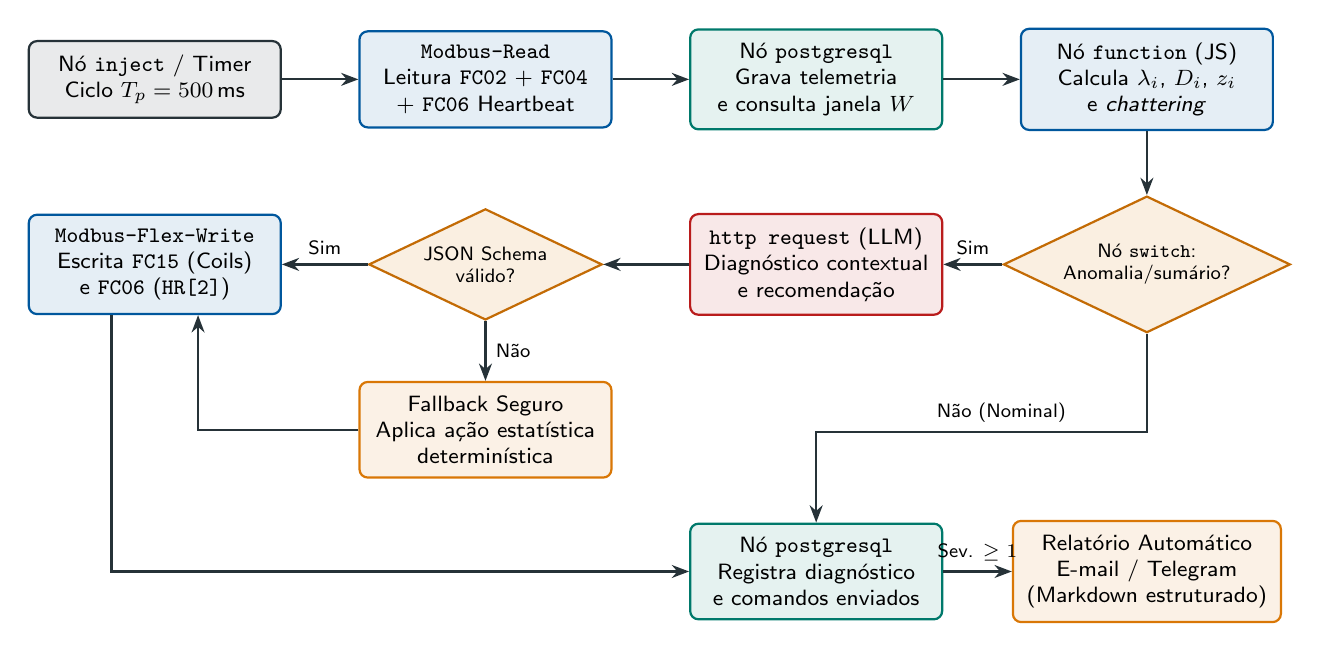
\begin{tikzpicture}[
    font=\sffamily\footnotesize,
    proc/.style={rectangle, rounded corners=3pt, draw=#1, fill=#1!10, thick, minimum width=3.2cm, minimum height=0.95cm, align=center, inner sep=5pt},
    dec/.style={diamond, aspect=2.1, draw=amberwarn!90!black, fill=amberwarn!12, thick, align=center, inner sep=2pt, font=\sffamily\scriptsize},
    arr/.style={-{Stealth[length=2.2mm]}, thick, draw=slateink}
  ]
    % Linha 1: Ingestão e Estatística (esquerda -> direita)
    \node[proc=slateink] (trig)   at (0,0)    {\textbf{Nó \texttt{inject} / Timer}\\Ciclo $T_p = 500\,\text{ms}$};
    \node[proc=wegblue]  (mbread) at (4.2,0)  {\textbf{\texttt{Modbus-Read}}\\Leitura \texttt{FC02} + \texttt{FC04}\\+ \texttt{FC06} Heartbeat};
    \node[proc=tealnode] (pgraw)  at (8.4,0)  {\textbf{Nó \texttt{postgresql}}\\Grava telemetria\\e consulta janela $W$};
    \node[proc=wegblue]  (stats)  at (12.6,0) {\textbf{Nó \texttt{function} (JS)}\\Calcula $\lambda_i$, $D_i$, $z_i$\\e \textit{chattering}};

    % Linha 2: Decisão, IA, Validação e Escrita (direita -> esquerda)
    \node[dec]               (decia)   at (12.6,-2.35) {Nó \texttt{switch}:\\Anomalia/sumário?};
    \node[proc=crimsonalert] (llm)     at (8.4,-2.35)  {\textbf{\texttt{http request} (LLM)}\\Diagnóstico contextual\\e recomendação};
    \node[dec]               (decjson) at (4.2,-2.35)  {JSON Schema\\válido?};
    \node[proc=wegblue]      (mbwrite) at (0,-2.35)    {\textbf{\texttt{Modbus-Flex-Write}}\\Escrita \texttt{FC15} (Coils)\\e \texttt{FC06} (\texttt{HR[2]})};

    % Linha 3: Fallback determinístico
    \node[proc=amberwarn]    (fallback) at (4.2,-4.45) {\textbf{Fallback Seguro}\\Aplica ação estatística\\determinística};

    % Linha 4: Auditoria e Relatórios Automáticos (sem cruzamentos)
    \node[proc=tealnode]     (pgdiag)   at (8.4,-6.25) {\textbf{Nó \texttt{postgresql}}\\Registra diagnóstico\\e comandos enviados};
    \node[proc=amberwarn]    (rep)      at (12.6,-6.25){\textbf{Relatório Automático}\\E-mail / Telegram\\(Markdown estruturado)};

    % Conexões Linha 1 -> Linha 2
    \draw[arr] (trig) -- (mbread);
    \draw[arr] (mbread) -- (pgraw);
    \draw[arr] (pgraw) -- (stats);
    \draw[arr] (stats) -- (decia);

    % Conexões Linha 2
    \draw[arr] (decia.west) -- node[above, font=\sffamily\scriptsize]{Sim} (llm.east);
    \draw[arr] (llm.west) -- (decjson.east);
    \draw[arr] (decjson.west) -- node[above, font=\sffamily\scriptsize]{Sim} (mbwrite.east);

    % Ramo Fallback (JSON inválido / timeout LLM)
    \draw[arr] (decjson.south) -- node[right, font=\sffamily\scriptsize]{Não} (fallback.north);
    \draw[arr] (fallback.west) -| ([xshift=0.55cm]mbwrite.south);

    % Ramo Auditoria pós-escrita Modbus (passa livre abaixo do Fallback)
    \draw[arr] ([xshift=-0.55cm]mbwrite.south) |- (pgdiag.west);

    % Ramo Nominal (sem invocação LLM) -> Auditoria
    \draw[arr] (decia.south) -- ++(0,-1.25) -| node[pos=0.22, above, font=\sffamily\scriptsize]{Não (Nominal)} (pgdiag.north);

    % Disparo de relatório automático
    \draw[arr] (pgdiag.east) -- node[above, font=\sffamily\scriptsize]{Sev. $\ge 1$} (rep.west);
  \end{tikzpicture}%
  }
  \fonte{Elaborado pelo autor (2026).}
\end{figure}

\section{Modelagem Estatística em Janela Temporal Deslizante}
\label{sec:nodered_estatistica}

A camada determinística avalia o comportamento dinâmico de cada sensor discreto $i \in \{1, 2, 3, 4\}$ sobre uma janela temporal deslizante de duração $W = 60\,\text{s}$ (equivalente a $K = W / T_p = 120$ amostras nominais). Três indicadores quantitativos são extraídos continuamente \cite{chandola_2009}:

\begin{enumerate}
  \item \textbf{Taxa de acionamento ($\lambda_i$):} obtida pela diferença modular do contador acumulado no CLP (\textit{Input Registers} \texttt{0..3}) entre o início e o término da janela, convertida em eventos por minuto:
  \begin{equation}
    \label{eq:taxa_acionamento}
    \lambda_i(W) = \frac{N_i(W)}{W} \times 60
  \end{equation}
  em que $N_i(W) = \left(C_i(t) - C_i(t - W)\right) \bmod 65536$ representa o total de bordas de subida observadas na janela.

  \item \textbf{Proporção de tempo ativo (\textit{duty cycle}, $D_i$):} quantifica a fração de amostras em que o sensor permaneceu em estado de alarme ou acionado:
  \begin{equation}
    \label{eq:duty_cycle}
    D_i(W) = \frac{1}{K} \sum_{k=1}^{K} s_{i,k}
  \end{equation}
  onde $s_{i,k} \in \{0, 1\}$ é o estado booleano filtrado do sensor $i$ na amostra $k$.

  \item \textbf{Escore padronizado de anomalia (\textit{Z-score}, $z_i$):} mede o afastamento da taxa atual de acionamentos em relação à linha de base histórica ($\mu_i, \sigma_i$) calculada sobre as últimas 24 horas de operação em regime nominal:
  \begin{equation}
    \label{eq:zscore}
    z_i(W) = \frac{\lambda_i(W) - \mu_i}{\sigma_i + \epsilon}
  \end{equation}
  sendo $\epsilon = 0{,}01\,\text{eventos/min}$ uma constante positiva de regularização que previne divisões por zero quando $\sigma_i = 0$.
\end{enumerate}

O critério estatístico classifica cada janela em quatro níveis de severidade padronizados, apresentados no Quadro~\ref{quadro:severidade}. Essa classificação determina simultaneamente o roteamento no nó \texttt{switch} para invocação do agente LLM e a ação de \textit{fallback} caso a camada cognitiva esteja indisponível.

\begin{quadro}[htb]
  \centering
  \SingleSpacing
  \caption{Matriz determinística de classificação de severidade e política de acionamento da camada híbrida}
  \label{quadro:severidade}
  \footnotesize
  \begin{tabularx}{\textwidth}{|p{1.9cm}|p{1.1cm}|L|p{3.9cm}|}
    \hline
    \textbf{Severidade} & \textbf{Código} & \textbf{Condição Estatística / Evento na Janela $W$} & \textbf{Ação no Node-RED e Atuadores} \\
    \hline
    \texttt{NORMAL} & \texttt{0} & $|z_1| < 2{,}0$; $D_2 = 0$; $D_3 = 0$; \texttt{DI3=1}; sem watchdog & Persistência regular; \texttt{L1=ON}, \texttt{L2=OFF}, \texttt{L3=OFF}; LLM apenas em sumário periódico \\
    \hline
    \texttt{ATENCAO} & \texttt{1} & $2{,}0 \le |z_1| < 3{,}0$ (desvio de cadência) ou $0 < D_2 < 0{,}30$ (nível alto intermitente) & Invoca agente LLM para diagnóstico; avalia acionamento preventivo de \texttt{L2}; registra alerta \\
    \hline
    \texttt{CRITICO} & \texttt{2} & $|z_1| \ge 3{,}0$ (\textit{chattering}/bloqueio), $D_2 \ge 0{,}30$, \texttt{DI2=1} (sobretemp.) ou watchdog ativo & Invoca agente LLM; comanda \texttt{L1=OFF}, \texttt{L2=ON}, \texttt{L3=ON}; dispara relatório imediato \\
    \hline
    \texttt{EMERGENCIA} & \texttt{3} & \texttt{DI3=0} ou \texttt{xFlag\_EmergTravada=1} & CLP já impõe veto local imediato; agente LLM gera relatório forense de incidente \\
    \hline
  \end{tabularx}
  \fonte{Elaborado pelo autor (2026).}
\end{quadro}

O Quadro~\ref{quadro:codigo_js} apresenta o código JavaScript de referência implementado no nó \texttt{function} do Node-RED para processar as linhas retornadas pelo PostgreSQL em \texttt{msg.payload}, ler a linha de base do contexto \texttt{flow}, computar as Equações~\eqref{eq:taxa_acionamento}--\eqref{eq:zscore} e preparar a mensagem para o nó \texttt{switch}.

\begin{quadro}[htb]
  \centering
  \SingleSpacing
  \caption{Código JavaScript do nó \texttt{function} no Node-RED para agregação temporal e detecção estatística}
  \label{quadro:codigo_js}
  \begin{lstlisting}[language=JavaScript]
// Entrada: msg.payload contendo array de amostras da janela W=60s vindo do no postgresql
const amostras = Array.isArray(msg.payload) ? msg.payload : [];
if (amostras.length === 0) {
  msg.payload = { status: "SEM_DADOS", acionar_llm: false };
  return msg;
}

const inicio = amostras[0];
const fim    = amostras[amostras.length - 1];
const K      = amostras.length;
const W_SEG  = 60;
const EPS    = 0.01;

// Diferenca modular segura para contadores Modbus UINT (16 bits)
const deltaMod16 = (atual, anterior) => (atual - anterior + 65536) % 65536;

const nPresenca  = deltaMod16(fim.cnt_presenca, inicio.cnt_presenca);
const taxaPres   = (nPresenca / W_SEG) * 60;
const dutyNivel  = amostras.reduce((acc, s) => acc + (s.di_nivel_alto ? 1 : 0), 0) / K;
const dutyTemp   = amostras.reduce((acc, s) => acc + (s.di_sobretemp  ? 1 : 0), 0) / K;
const emergAtiva = fim.flag_emerg_travada || !fim.di_emergencia_ok;

// Parametros de baseline lidos do contexto de fluxo (flow) ou da consulta SQL
const baseCtx   = flow.get("baseline_presenca") || { mu: 12.0, sigma: 2.5 };
const muPres    = Number(fim.baseline_mu_presenca ?? baseCtx.mu);
const sigmaPres = Number(fim.baseline_sigma_presenca ?? baseCtx.sigma);
const zPresenca = (taxaPres - muPres) / (sigmaPres + EPS);

// Classificacao deterministica de severidade e acao de fallback
let severidade = 0; // 0=NORMAL, 1=ATENCAO, 2=CRITICO, 3=EMERGENCIA
let fallbackCmd = { cmd_motor: true, cmd_valvula: false, cmd_alarme: false };

if (emergAtiva) {
  severidade = 3;
  fallbackCmd = { cmd_motor: false, cmd_valvula: false, cmd_alarme: true };
} else if (dutyTemp > 0 || dutyNivel >= 0.30 || Math.abs(zPresenca) >= 3.0 || fim.flag_watchdog) {
  severidade = 2;
  fallbackCmd = { cmd_motor: false, cmd_valvula: true, cmd_alarme: true };
} else if (dutyNivel > 0 || Math.abs(zPresenca) >= 2.0) {
  severidade = 1;
  fallbackCmd = { cmd_motor: true, cmd_valvula: true, cmd_alarme: false };
}

msg.payload = {
  janela_inicio: inicio.capturado_em,
  janela_fim: fim.capturado_em,
  amostras_k: K,
  taxa_presenca_min: Number(taxaPres.toFixed(2)),
  duty_nivel: Number(dutyNivel.toFixed(3)),
  duty_sobretemp: Number(dutyTemp.toFixed(3)),
  zscore_presenca: Number(zPresenca.toFixed(2)),
  estado_clp: fim.estado_clp,
  cod_intertravamento: fim.cod_intertrav,
  severidade_estatistica: severidade,
  fallback_comandos: fallbackCmd,
  acionar_llm: severidade >= 1 || flow.get("ciclo_sumario_horario") === true
};
return msg;
  \end{lstlisting}
  \fonte{Elaborado pelo autor (2026).}
\end{quadro}

\section{Camada Cognitiva (Agente LLM), Governança por JSON Schema e Relatórios}
\label{sec:nodered_ia}

Quando \texttt{msg.payload.acionar\_llm} assume valor verdadeiro, o nó \texttt{switch} direciona a mensagem para o ramo cognitivo, onde um nó \texttt{function} monta o \textit{prompt} estruturado contendo o resumo estatístico da janela, o estado atual do PLC500 e os últimos cinco eventos do PostgreSQL, enviando-o via nó \textbf{\texttt{http request}} à API do modelo de linguagem \cite{nodered_docs}. Essa arquitetura suporta tanto provedores em nuvem quanto servidores de inferência locais na rede interna, impondo três salvaguardas obrigatórias:

\begin{enumerate}
  \item \textbf{Restrição estrutural por \textit{JSON Schema}:} o nó validador JSON do Node-RED confronta a resposta do modelo com o esquema especificado no Quadro~\ref{quadro:json_schema} (\texttt{additionalProperties: false}, tipos booleanos estritos para os comandos de LEDs e enumeração fechada de severidade).
  \item \textbf{Regra de monotonicidade de segurança:} o nó \texttt{function} pós-validação impede que o modelo rebaixe uma severidade estatística \texttt{CRITICO} ou \texttt{EMERGENCIA} para \texttt{NORMAL} e bloqueia qualquer comando \texttt{cmd\_motor = true} enquanto houver sobretemperatura, nível alto sustentado ou emergência travada, formatando em seguida o payload para o nó \texttt{Modbus-Flex-Write} (\texttt{fc: 15, address: 0, quantity: 3}).
  \item \textbf{Relatório técnico automatizado:} nos eventos com severidade $\ge 1$ ou nos fechamentos periódicos de turno, os campos \texttt{diagnostico}, \texttt{causa\_provavel} e \texttt{resumo\_executivo} são formatados em Markdown por um nó \texttt{template} e despachados automaticamente por e-mail ou Telegram aos operadores.
\end{enumerate}

\begin{quadro}[htb]
  \centering
  \SingleSpacing
  \caption{\textit{JSON Schema} obrigatório de validação da saída do agente LLM no Node-RED}
  \label{quadro:json_schema}
  \begin{lstlisting}[language=JSON]
{
  "$schema": "https://json-schema.org/draft/2020-12/schema",
  "title": "DiagnosticoAtuacaoPLC500",
  "type": "object",
  "additionalProperties": false,
  "required": [
    "severidade", "diagnostico", "causa_provavel",
    "comandos_atuadores", "requer_relatorio", "resumo_executivo"
  ],
  "properties": {
    "severidade": {
      "type": "string",
      "enum": ["NORMAL", "ATENCAO", "CRITICO", "EMERGENCIA"]
    },
    "diagnostico": { "type": "string", "minLength": 10, "maxLength": 400 },
    "causa_provavel": { "type": "string", "minLength": 5, "maxLength": 250 },
    "comandos_atuadores": {
      "type": "object",
      "additionalProperties": false,
      "required": ["cmd_motor", "cmd_valvula", "cmd_alarme"],
      "properties": {
        "cmd_motor":   { "type": "boolean" },
        "cmd_valvula": { "type": "boolean" },
        "cmd_alarme":  { "type": "boolean" }
      }
    },
    "requer_relatorio": { "type": "boolean" },
    "resumo_executivo": { "type": "string", "minLength": 20, "maxLength": 800 }
  }
}
  \end{lstlisting}
  \fonte{Elaborado pelo autor (2026).}
\end{quadro}

\section{Persistência e Rastreabilidade em PostgreSQL}
\label{sec:nodered_postgres}

Para assegurar rastreabilidade forense completa das leituras e decisões automatizadas, utiliza-se o banco de dados relacional \textbf{PostgreSQL} acessado a partir do Node-RED \cite{postgresql_docs}. O esquema relacional separa telemetria bruta de alta cadência, métricas agregadas por janela, diagnósticos emitidos pelo agente LLM (registrando explicitamente quando o \textit{fallback} estatístico foi utilizado) e trilha de auditoria dos comandos escritos via \texttt{Modbus-Flex-Write}. O script DDL completo é apresentado no Quadro~\ref{quadro:ddl_sql}.

\begin{quadro}[htb]
  \centering
  \SingleSpacing
  \caption{Script DDL SQL (PostgreSQL) da base de telemetria, análise híbrida e auditoria de atuação}
  \label{quadro:ddl_sql}
  \begin{lstlisting}[language=PGSQL]
CREATE TABLE IF NOT EXISTS telemetria_sensores (
  id                  BIGSERIAL PRIMARY KEY,
  capturado_em        TIMESTAMPTZ NOT NULL DEFAULT NOW(),
  di_presenca         BOOLEAN NOT NULL,
  di_nivel_alto       BOOLEAN NOT NULL,
  di_sobretemp        BOOLEAN NOT NULL,
  di_emergencia_ok    BOOLEAN NOT NULL,
  flag_emerg_travada  BOOLEAN NOT NULL,
  flag_watchdog       BOOLEAN NOT NULL,
  cnt_presenca        INTEGER NOT NULL,
  cnt_nivel_alto      INTEGER NOT NULL,
  cnt_sobretemp       INTEGER NOT NULL,
  estado_clp          SMALLINT NOT NULL,
  mascara_do_real     SMALLINT NOT NULL,
  cod_intertrav       SMALLINT NOT NULL
);
CREATE INDEX IF NOT EXISTS idx_tel_capturado ON telemetria_sensores (capturado_em DESC);

CREATE TABLE IF NOT EXISTS janelas_analiticas (
  id                     BIGSERIAL PRIMARY KEY,
  janela_inicio          TIMESTAMPTZ NOT NULL,
  janela_fim             TIMESTAMPTZ NOT NULL,
  amostras_k             INTEGER NOT NULL,
  taxa_presenca_min      DOUBLE PRECISION NOT NULL,
  duty_nivel             DOUBLE PRECISION NOT NULL,
  duty_sobretemp         DOUBLE PRECISION NOT NULL,
  zscore_presenca        DOUBLE PRECISION NOT NULL,
  severidade_estatistica SMALLINT NOT NULL CHECK (severidade_estatistica BETWEEN 0 AND 3)
);

CREATE TABLE IF NOT EXISTS diagnosticos_ia (
  id                 BIGSERIAL PRIMARY KEY,
  janela_id          BIGINT NOT NULL REFERENCES janelas_analiticas (id),
  criado_em          TIMESTAMPTZ NOT NULL DEFAULT NOW(),
  severidade_final   VARCHAR(16) NOT NULL,
  origem_decisao     VARCHAR(16) NOT NULL CHECK (origem_decisao IN ('LLM', 'FALLBACK_STATS')),
  diagnostico        TEXT NOT NULL,
  causa_provavel     TEXT NOT NULL,
  payload_validado   JSONB NOT NULL,
  relatorio_enviado  BOOLEAN NOT NULL DEFAULT FALSE
);

CREATE TABLE IF NOT EXISTS comandos_atuadores (
  id                 BIGSERIAL PRIMARY KEY,
  diagnostico_id     BIGINT REFERENCES diagnosticos_ia (id),
  enviado_em         TIMESTAMPTZ NOT NULL DEFAULT NOW(),
  cmd_motor          BOOLEAN NOT NULL,
  cmd_valvula        BOOLEAN NOT NULL,
  cmd_alarme         BOOLEAN NOT NULL,
  severidade_hr2     SMALLINT NOT NULL,
  mascara_do_confirm SMALLINT,
  veto_local_clp     BOOLEAN NOT NULL DEFAULT FALSE
);
  \end{lstlisting}
  \fonte{Elaborado pelo autor (2026).}
\end{quadro}

Com o índice decrescente em \texttt{capturado\_em}, as consultas de janela deslizante de 60 segundos executadas pelos nós do Node-RED mantêm tempo de resposta baixo e previsível, facilitando também a conexão de dashboards operacionais.

% ==============================================================================
% capitulos/06_plano_validacao.tex
% Capítulo 6 — Plano de Validação, Critérios de Aceitação e Análise de Riscos
% ==============================================================================

\chapter{Plano de Validação, Critérios de Aceitação e Análise de Riscos}
\label{cap:plano_validacao}

Em coerência com a delimitação estabelecida na Seção~\ref{sec:escopo}, este capítulo especifica o protocolo formal de validação em bancada, os casos de teste obrigatórios, os critérios quantitativos de aceitação e a matriz de análise e mitigação de riscos técnicos para o comissionamento do sistema.

\section{Configuração do Ambiente de Ensaios em Bancada}
\label{sec:val_ambiente}

A validação integral da arquitetura deve ser conduzida em bancada didático-industrial composta por:
\begin{itemize}
  \item Um controlador \textbf{WEG PLC500} alimentado em 24\,Vcc, com o programa \texttt{PLC\_PRG} (Quadro~\ref{quadro:codigo_st}) carregado via interface \texttt{ETH1} (\texttt{192.168.20.10}) e servidor Modbus TCP/IP ativo em \texttt{ETH2} (\texttt{192.168.10.10:502}).
  \item Quatro botoeiras industriais (três NA em \texttt{DI0}--\texttt{DI2} e uma botoeira tipo cogumelo com trava NF em \texttt{DI3}) e quatro sinalizadores LED de 24\,Vcc conectados em \texttt{DO0}--\texttt{DO3}, conforme a Tabela~\ref{tab:mapeamento_io}.
  \item Um servidor local (\texttt{192.168.10.20}) executando \textbf{Node-RED} com os pacotes \texttt{node-red-contrib-modbus} e \texttt{node-red-contrib-postgresql}, banco de dados \textbf{PostgreSQL} inicializado com o DDL do Quadro~\ref{quadro:ddl_sql} e conectividade configurada para o endpoint LLM utilizado pelo nó \texttt{http request}.
  \item Parâmetros nominais de ensaio: ciclo do CLP de $10\,\text{ms}$, \textit{debounce} $T_{db} = 50\,\text{ms}$, \textit{polling} Modbus $T_p = 500\,\text{ms}$, janela deslizante $W = 60\,\text{s}$ e \textit{watchdog} $T_{wd} = 5000\,\text{ms}$.
\end{itemize}

\section{Casos de Teste Funcionais, Analíticos e de Segurança}
\label{sec:val_casos}

O Quadro~\ref{quadro:casos_teste} especifica os dez casos de teste obrigatórios (\texttt{CT-01} a \texttt{CT-10}) que cobrem aquisição de sensores, atuação remota pelos nós do Node-RED, persistência SQL, detecção estatística, diagnóstico assistido por IA, resiliência a falhas de contrato JSON, precedência do intertravamento local de segurança e perda de comunicação de rede.

\begin{quadro}[htb]
  \centering
  \SingleSpacing
  \caption{Protocolo de casos de teste funcionais, analíticos e de segurança para validação em bancada}
  \label{quadro:casos_teste}
  \scriptsize
  \begin{tabularx}{\textwidth}{|p{1.05cm}|p{2.45cm}|L|L|}
    \hline
    \textbf{ID} & \textbf{Cenário} & \textbf{Procedimento de Estímulo em Bancada} & \textbf{Resultado Esperado (Critério de Aprovação)} \\
    \hline
    \texttt{CT-01} & Aquisição e \textit{debounce} das botoeiras & Acionar \texttt{B1}--\texttt{B3} com pulsos curtos ($< 30\,\text{ms}$) e pulsos válidos ($\ge 100\,\text{ms}$), monitorando \texttt{Modbus-Read} (\texttt{FC02}/\texttt{FC04}). & Pulsos $< 50\,\text{ms}$ são rejeitados sem incrementar contadores; pulsos válidos atualizam \texttt{DI0}--\texttt{DI2} e \texttt{IR[0..2]} exatamente em $+1$. \\
    \hline
    \texttt{CT-02} & Atuação remota nos LEDs via Node-RED & Em estado \texttt{NORMAL\_AUTO} (\texttt{HabRemoto=1}), enviar \texttt{Coils 0..2} via \texttt{Modbus-Flex-Write} (\texttt{FC15}) alternando \texttt{L1}--\texttt{L3}. & LEDs físicos refletem os comandos em até um ciclo de \textit{polling}; \texttt{IR[5]} (\texttt{wMascara\_DO\_Real}) coincide integralmente com os \textit{Coils}. \\
    \hline
    \texttt{CT-03} & Persistência de séries temporais & Manter o fluxo Node-RED ativo por 10 minutos contínuos com acionamentos regulares em \texttt{B1}. & Aproximadamente 1200 registros gravados em \texttt{telemetria\_sensores} sem lacunas superiores a $2\,T_p$ e sem erros de integridade SQL. \\
    \hline
    \texttt{CT-04} & Detecção estatística de \textit{chattering} & Pressionar \texttt{B1} repetidamente acima da linha de base ($\mu_1 + 3\sigma_1$) dentro de uma janela $W = 60\,\text{s}$. & Nó \texttt{function} calcula $|z_1| \ge 3{,}0$, eleva \texttt{severidade\_estatistica = 2}, grava \texttt{janelas\_analiticas} e aciona o ramo LLM via nó \texttt{switch}. \\
    \hline
    \texttt{CT-05} & Diagnóstico IA com \textit{JSON Schema} & Sustentar \texttt{B2} (nível alto) por $\ge 20\,\text{s}$ na janela $W$ e inspecionar a resposta do ramo LLM no Node-RED. & Resposta validada contra o Quadro~\ref{quadro:json_schema}, \texttt{origem\_decisao='LLM'}, comando \texttt{L2=ON} e \texttt{L3=ON} escritos via Modbus e auditados. \\
    \hline
    \texttt{CT-06} & \textit{Fallback} por falha ou violação JSON & Injetar resposta malformada ou simular \textit{timeout} no nó \texttt{http request} durante anomalia ativa em \texttt{B2}. & Validador JSON desvia para o ramo de \textit{fallback}, registra \texttt{FALLBACK\_STATS} e aplica comandos determinísticos seguros nos LEDs. \\
    \hline
    \texttt{CT-07} & Precedência local da parada de emergência & Com \texttt{L1=ON} comandado pelo Node-RED, pressionar a botoeira NF \texttt{B4\_Emergencia} (ou abrir o fio de \texttt{DI3}) e enviar \texttt{cmd\_motor=TRUE}. & PLC500 desliga \texttt{L1} e \texttt{L2}, acende \texttt{L3}, apaga \texttt{L4} em $\le 20\,\text{ms}$, trava \texttt{uiEstado\_CLP=4} e ignora comandos remotos até rearme seguro. \\
    \hline
    \texttt{CT-08} & Proteção térmica local (\texttt{DI2}) & Acionar \texttt{B3\_SensSobretemp} enquanto o Node-RED solicita \texttt{cmd\_motor=TRUE} e \texttt{cmd\_valvula=FALSE}. & PLC500 veta o motor (\texttt{L1=OFF}), força válvula de resfriamento (\texttt{L2=ON}) e alarme (\texttt{L3=ON}), reportando \texttt{uiCod\_Intertrav=2}. \\
    \hline
    \texttt{CT-09} & Perda física de rede e \textit{watchdog} & Com sistema em \texttt{NORMAL\_AUTO} e \texttt{L1=ON}, desconectar fisicamente o cabo Ethernet da porta \texttt{ETH2}. & Em no máximo $T_{wd} = 5\,\text{s}$, CLP entra em \texttt{MODO\_DEGRADADO} (\texttt{uiEstado\_CLP=3}), desliga \texttt{L1}/\texttt{L4} e acende \texttt{L3}; reconexão restaura operação. \\
    \hline
    \texttt{CT-10} & Relatório automático de incidente & Disparar evento crítico (\texttt{CT-05} ou \texttt{CT-07}) com canal de notificação habilitado no Node-RED. & Relatório Markdown contendo janela, métricas, diagnóstico e ações é entregue no canal configurado e marcado como \texttt{relatorio\_enviado=TRUE}. \\
    \hline
  \end{tabularx}
  \fonte{Elaborado pelo autor (2026).}
\end{quadro}

\section{Critérios Quantitativos de Aceitação}
\label{sec:val_criterios}

Além da aprovação qualitativa nos dez casos de teste do Quadro~\ref{quadro:casos_teste}, o comissionamento completo da bancada condiciona-se ao atendimento simultâneo das metas quantitativas especificadas na Tabela~\ref{tab:criterios_aceitacao}.

\begin{table}[htb]
  \centering
  \SingleSpacing
  \caption{Critérios quantitativos de aceitação para aprovação da arquitetura em bancada}
  \label{tab:criterios_aceitacao}
  \footnotesize
  \begin{tabularx}{\textwidth}{@{}p{3.8cm}p{2.4cm}p{2.3cm}L@{}}
    \toprule
    \textbf{Indicador de Desempenho} & \textbf{Meta de Aceitação} & \textbf{Casos Vinculados} & \textbf{Método de Medição na Bancada} \\
    \midrule
    Tempo de resposta do intertravamento local (\texttt{DI3}/\texttt{DI2} $\rightarrow$ \texttt{DO}) & $\le 20\,\text{ms}$ ($\le 2$ ciclos CLP) & \texttt{CT-07}, \texttt{CT-08} & Registro interno de \textit{timestamp} no CODESYS Trace \\
    Latência RTT média de leitura/escrita Modbus TCP (\texttt{ETH2}) & $\le 50\,\text{ms}$ (p95 $\le 150\,\text{ms}$) & \texttt{CT-01}, \texttt{CT-02} & Medição de tempo entre disparo e resposta em nó \texttt{function} no Node-RED \\
    Tempo de detecção de perda de enlace pelo \textit{watchdog} & $5{,}0\,\text{s} \pm 0{,}2\,\text{s}$ & \texttt{CT-09} & Cronometragem entre desconexão física de \texttt{ETH2} e desligamento de \texttt{DO0}/\texttt{DO3} \\
    Conformidade de contrato \textit{JSON Schema} antes da escrita Modbus & $100\%$ (zero exceções) & \texttt{CT-05}, \texttt{CT-06} & Auditoria na tabela \texttt{diagnosticos\_ia} e logs do validador no Node-RED \\
    Atuações indevidas de \texttt{L1} em emergência ou sobretemperatura & $0$ ocorrências & \texttt{CT-07}, \texttt{CT-08} & Consulta SQL verificando \texttt{mascara\_do\_real} quando \texttt{cod\_intertrav} $\in \{1,2\}$ \\
    Disponibilidade de ingestão em regime contínuo (10\,min) & $\ge 99{,}0\%$ das amostras & \texttt{CT-03} & Contagem de registros em \texttt{telemetria\_sensores} vs.\ esperado ($1200$) \\
    Latência fim a fim da geração de relatório automático (com LLM) & $\le 15\,\text{s}$ após evento & \texttt{CT-10} & Diferença entre \texttt{janela\_fim} e carimbo de entrega da notificação \\
    \bottomrule
  \end{tabularx}
  \fonte{Elaborado pelo autor (2026).}
\end{table}

\section{Análise de Riscos Técnicos e Estratégias de Mitigação}
\label{sec:val_riscos}

A integração entre protocolos industriais legados e agentes baseados em IA exige tratamento explícito de riscos de segurança funcional, cibersegurança e confiabilidade de software \cite{stouffer_nist_ot, iec_62443}. O Quadro~\ref{quadro:riscos} cataloga os principais riscos identificados no projeto e as salvaguardas arquiteturais incorporadas para mitigá-los.

\begin{quadro}[htb]
  \centering
  \SingleSpacing
  \caption{Matriz de análise de riscos técnicos e mecanismos de mitigação incorporados ao projeto}
  \label{quadro:riscos}
  \scriptsize
  \begin{tabularx}{\textwidth}{|p{2.6cm}|p{1.3cm}|L|L|}
    \hline
    \textbf{Risco Identificado} & \textbf{Impacto} & \textbf{Causa Raiz Potencial} & \textbf{Mitigação Arquitetural Adotada} \\
    \hline
    Acesso não autorizado à porta TCP~502 (Modbus sem TLS) & Alto & Protocolo Modbus TCP/IP trafega em texto claro e sem autenticação nativa. & Isolamento físico na interface \texttt{ETH2} em VLAN/sub-rede dedicada, firewall permitindo apenas IP \texttt{192.168.10.20} e migração futura para OPC~UA/TLS. \\
    \hline
    Alucinação ou comando inseguro pelo agente LLM & Alto & Natureza probabilística de modelos de linguagem ou variações de resposta de API. & Validação obrigatória por \textit{JSON Schema} no Node-RED, regra de monotonicidade, \textit{fallback} estatístico e veto físico determinístico no WEG PLC500. \\
    \hline
    Perda de conectividade ou travamento do host Node-RED & Alto & Queda de cabo Ethernet, reinicialização do servidor IT ou indisponibilidade do serviço. & Mecanismo de \textit{heartbeat} em \texttt{HR[0]} com \textit{watchdog} de $5\,\text{s}$ no PLC500 forçando desligamento do motor e sinalização de alarme. \\
    \hline
    Falsos disparos por trepidação mecânica das botoeiras & Médio & Repique elétrico (\textit{bouncing}) de contatos mecânicos nas entradas \texttt{DI0}--\texttt{DI2}. & Filtro \textit{debounce} por temporizador \texttt{TON} de $50\,\text{ms}$ no CLP e contadores baseados em detecção de borda filtrada (\texttt{R\_TRIG}). \\
    \hline
    Rompimento de fiação da parada de emergência & Crítico & Desconexão acidental de borne ou rompimento de condutor em \texttt{DI3}. & Adoção de lógica Normalmente Fechada (NF) \textit{fail-safe} sem retardo de energização e travamento com rearme explícito. \\
    \hline
    Crescimento excessivo da tabela de telemetria & Baixo & Gravação contínua a cada $500\,\text{ms}$ ($\approx 172{,}8\,\text{mil}$ linhas por dia). & Índice temporal decrescente no PostgreSQL e recomendação de política de retenção ou particionamento diário em operação prolongada. \\
    \hline
  \end{tabularx}
  \fonte{Elaborado pelo autor (2026).}
\end{quadro}

% ==============================================================================
% capitulos/07_consideracoes_finais.tex
% Capítulo 7 — Considerações Finais e Trabalhos Futuros
% ==============================================================================

\chapter{Considerações Finais e Trabalhos Futuros}
\label{cap:consideracoes}

\section{Síntese dos Resultados de Projeto}
\label{sec:cons_sintese}

Este documento técnico apresentou a arquitetura, a especificação e a implementação de referência de uma pipeline híbrida de análise de dados industriais integrando o controlador lógico programável \textbf{WEG PLC500}, o protocolo \textbf{Modbus TCP/IP} e a plataforma \textbf{Node-RED}, desenvolvida como entrega de uma \textbf{Situação de Aprendizagem (SA) de IoT de escopo livre}. A definição desse escopo representou uma evolução pragmática e metodologicamente validada a partir da concepção inicial do projeto --- que previa um servidor de tempo NTPv4 baseado em antena GNSS e microcontrolador ESP32, mas esbarrou na inviabilidade física de recepção satelital em laboratório \textit{indoor}. A realização da pivotagem mediante \textbf{aprovação prévia do professor} garantiu a integral conformidade do projeto com o estabelecido na atividade acadêmica, resultando em uma bancada de Internet Industrial das Coisas (IIoT) autocontida, reproduzível e independente de infraestrutura externa de radiofrequência.

Utilizando quatro botoeiras (simulando sensores de presença, nível crítico, sobretemperatura e parada de emergência NF) e quatro sinalizadores LED (simulando motor, válvula de alívio, alarme e indicador de operação normal), a arquitetura projetada demonstra como conciliar ferramentas de fluxo de eventos e modelos de IA com requisitos estritos de engenharia de controle:
\begin{itemize}
  \item \textbf{Determinismo preservado na camada OT:} a lógica em \textit{Structured Text} (IEC 61131-3) no CODESYS V3.5 garante filtragem de \textit{debounce}, contagem precisa de eventos, supervisão de enlace via \textit{watchdog} de \textit{heartbeat} e intertravamento local \textit{fail-safe} com precedência absoluta sobre comandos remotos.
  \item \textbf{Interoperabilidade transparente via Modbus TCP/IP e Node-RED:} o uso do pacote \texttt{node-red-contrib-modbus} aliado a um mapa de registradores base zero com palavra de retorno das saídas físicas (\texttt{wMascara\_DO\_Real}) assegura auditabilidade completa da malha fechada.
  \item \textbf{Inteligência analítica governada na camada IT:} a combinação entre estatística determinística em janelas deslizantes ($\lambda_i$, $D_i$ e \textit{Z-score}) em nós \texttt{function} e diagnóstico contextual por agente LLM protegido por \textit{JSON Schema} e política de \textit{fallback} evita o acoplamento direto de respostas probabilísticas a atuadores físicos, além de automatizar relatórios técnicos e a rastreabilidade em PostgreSQL.
  \item \textbf{Rigor metodológico na validação:} o protocolo formal de dez casos de teste, os critérios quantitativos de aceitação e a matriz de riscos oferecem um roteiro objetivo para o comissionamento da bancada.
\end{itemize}

\section{Limitações Conhecidas e Trabalhos Futuros}
\label{sec:cons_futuros}

Por empregar exclusivamente entradas e saídas digitais simuladas por botoeiras e LEDs nesta primeira etapa, o projeto concentra-se na dinâmica de eventos discretos e na validação arquitetural da malha OT/IT. Como desdobramentos naturais para trabalhos futuros, destacam-se:

\begin{enumerate}
  \item \textbf{Execução da campanha experimental em bancada:} implantar o sistema conforme o Apêndice~\ref{ap:checklist}, executar os casos \texttt{CT-01} a \texttt{CT-10} e registrar as medições reais de bancada (distribuição de latência RTT nos nós do Node-RED, tempo de resposta do intertravamento no CODESYS Trace e avaliação qualitativa dos diagnósticos emitidos pelo LLM).
  \item \textbf{Expansão para grandezas analógicas reais:} incorporar cartões de expansão da série MOD (compatíveis com a linha RUW100 do WEG PLC500) para leitura de sinais contínuos ($4\text{--}20\,\text{mA}$, $0\text{--}10\,\text{V}$ e termorresistências PT100), ampliando a camada analítica no Node-RED com técnicas multivariadas (\textit{Isolation Forest} ou EWMA).
  \item \textbf{Fortalecimento de cibersegurança no transporte:} avaliar a migração da comunicação supervisória para \textbf{OPC~UA com assinatura digital e criptografia TLS} --- suportado tanto no CODESYS do WEG PLC500 quanto no ecossistema Node-RED --- reduzindo a superfície de exposição associada ao Modbus TCP/IP em redes ampliadas \cite{stouffer_nist_ot, iec_62443}.
  \item \textbf{Observabilidade visual e sincronismo de tempo na rede OT:} integrar painéis gráficos diretamente à base PostgreSQL (via Grafana ou Node-RED Dashboard) e, caso futuramente se disponha de acesso a antena externa em topo de edifício, reintegrar o conceito original do servidor NTP Stratum~1 (ESP32 + GNSS) como fonte local de sincronismo de tempo para o WEG PLC500 e para o servidor Node-RED na sub-rede isolada \cite{rfc5905_ntp}.
\end{enumerate}


% ------------------------------------------------------------------------------
% ELEMENTOS PÓS-TEXTUAIS
% ------------------------------------------------------------------------------
\postextual

% Referências bibliográficas (abntex2-alf)
\bibliography{referencias}

% Apêndices
\begin{apendicesenv}
  \partapendices
  % ==============================================================================
% apendices/apendice_a_checklist.tex
% Apêndice A — Checklist de Comissionamento e Implantação em Bancada
% ==============================================================================

\chapter{Checklist de Comissionamento e Implantação em Bancada}
\label{ap:checklist}

Este apêndice consolida a sequência operacional recomendada para montagem, configuração inicial e verificação pré-ensaio da bancada envolvendo o controlador WEG PLC500, o ambiente CODESYS V3.5, o banco PostgreSQL e o fluxo no Node-RED.

\section{Etapa 1 -- Montagem Elétrica e Verificação de Hardware}
\begin{enumerate}
  \item Confirmar alimentação regulada de 24\,Vcc no WEG PLC500 e proteção por disjuntor/fusível adequado à bancada didática.
  \item Conectar as botoeiras NA em \texttt{DI0} (\texttt{\%IX0.0}), \texttt{DI1} (\texttt{\%IX0.1}) e \texttt{DI2} (\texttt{\%IX0.2}) em configuração PNP (comutando $+24\,\text{Vcc}$ para a entrada).
  \item Conectar a botoeira de emergência NF em \texttt{DI3} (\texttt{\%IX0.3}), confirmando presença de nível lógico alto (LED indicador da entrada aceso no CLP) em condição de repouso.
  \item Conectar os quatro sinalizadores LED de 24\,Vcc (ou LEDs discretos com resistores limitadores de $1{,}8\text{--}2{,}2\,\text{k}\Omega$) nas saídas \texttt{DO0}--\texttt{DO3} (\texttt{\%QX0.0}--\texttt{\%QX0.3}) referenciados ao $0\,\text{Vcc}$.
  \item Conectar o cabo Ethernet de engenharia à porta \texttt{ETH1} e o cabo da sub-rede Modbus dedicada à porta \texttt{ETH2}.
\end{enumerate}

\section{Etapa 2 -- Configuração do WEG PLC500 no CODESYS V3.5}
\begin{enumerate}
  \item Configurar o IP estático \texttt{192.168.20.10/24} na interface \texttt{ETH1} e \texttt{192.168.10.10/24} na interface \texttt{ETH2}.
  \item Inserir \texttt{Ethernet\_ETH2} e o dispositivo filho \texttt{ModbusTCP\_Server\_Device} (porta \texttt{502}, \textit{Unit ID} \texttt{1}) na árvore de dispositivos.
  \item Mapear integralmente os endereços base zero conforme a Tabela~\ref{tab:mapa_modbus}, habilitando a opção de atualização contínua das variáveis no ciclo de \texttt{MainTask} ($10\,\text{ms}$).
  \item Compilar sem erros, realizar \textit{download} de \texttt{PLC\_PRG} (Quadro~\ref{quadro:codigo_st}), colocar o CLP em modo \texttt{RUN} e verificar \texttt{uiVersao\_Mapa = 100} no registrador \texttt{HR[3]}.
\end{enumerate}

\section{Etapa 3 -- Implantação do PostgreSQL e do Fluxo Node-RED}
\begin{enumerate}
  \item No servidor \texttt{192.168.10.20}, verificar conectividade ICMP/TCP na porta \texttt{502} com \texttt{192.168.10.10} e confirmar regra de firewall restringindo a porta 502 apenas ao host do Node-RED.
  \item Criar a base de dados PostgreSQL dedicada e executar o script DDL do Quadro~\ref{quadro:ddl_sql}, validando a criação das quatro tabelas e do índice \texttt{idx\_tel\_capturado}.
  \item No gerenciador de paleta do Node-RED (\textit{Manage Palette}), instalar os pacotes \texttt{node-red-contrib-modbus} e \texttt{node-red-contrib-postgresql}, configurando o nó \texttt{Modbus-Client} (\texttt{192.168.10.10:502}, \textit{Unit ID}~\texttt{1}, \textit{timeout}~$1500\,\text{ms}$).
  \item Estruturar o fluxo conforme a Figura~\ref{fig:fluxo-pipeline-nodered}, inserindo o código JavaScript do Quadro~\ref{quadro:codigo_js} no nó \texttt{function} de análise temporal e o contrato do Quadro~\ref{quadro:json_schema} no nó validador JSON após o nó \texttt{http request}.
  \item Ativar o modo remoto (\texttt{Coil[4] = TRUE}), confirmar o acendimento do indicador \texttt{L4\_StatusOper} (\texttt{DO3}) e iniciar sequencialmente a execução dos casos de teste \texttt{CT-01} a \texttt{CT-10} do Quadro~\ref{quadro:casos_teste}.
\end{enumerate}

\end{apendicesenv}

\end{document}
